\documentclass[12pt, a4paper]{article}

%<<<===Переменные титульного листа
\newcommand{\kafedra}{ИИТ} % Кафедра X

\newcommand{\numberOfLab}{11-12-13-14} % Лабораторная работа №X
\newcommand{\semestr}{2} % За X семестр
\newcommand{\distiplina}{ОАиП} % По дисциплине <<X>>
\newcommand{\labTitle}{Исходный код} % Тема: <<X>>

% Выполнил
\newcommand{\kurs}{1} % Студент X курса
\newcommand{\group}{ПО-4 (1)} % группы X
\newcommand{\labAuthor}{Галанин П. И.} % X

% Проверил
\newcommand{\teacherStatus}{ст. преподаватель} % X
\newcommand{\teacher}{Хацкевич М. В.} % X

\newcommand{\labDate}{Брест, 2020} % X
%===>>>

%<<<===
\usepackage{../../../sty/encoding} % кодировка
\usepackage{../../../sty/titlePage} % титульный лист
\usepackage{../../../sty/fields} % поля
\usepackage{../../../sty/imgs} % картинки
\usepackage{../../../sty/code} % исходный код
\usepackage{../../../sty/labData} % для лабораторной
%===>>>

\begin{document}

%<<<===Титульный лист
\maketitle
\setcounter{page}{2}
%===>>>

%<<<===Содержание
\renewcommand{\contentsname}{Содержание}
\tableofcontents
\newpage
%===>>>

%<<<===ЛР
\labheading
%===>>>

%<<<===Цель
%\labgoal{}
%===>>>

%<<<===Ход Работы
\labreport
%===>>>

%<<<===Условие
\section{Структура проекта}
\begin{verbatim}
.
├── Makefile
└── src
    ├── lab
    │   ├── lab.c     
    │   ├── lab.drawio
    │   ├── lab.h     
    │   ├── lab.png   
    │   ├── lab.tex   
    │   └── menu
    │       ├── del_data
    │       │   ├── del_data.c     
    │       │   ├── del_data.drawio
    │       │   ├── del_data.h     
    │       │   ├── del_data.png
    │       │   └── del_data.tex
    │       ├── input_data
    │       │   ├── input_data.c
    │       │   ├── input_data.drawio
    │       │   ├── input_data.h
    │       │   ├── input_data.png
    │       │   └── input_data.tex
    │       ├── menu.c
    │       ├── menu.drawio
    │       ├── menu.h
    │       ├── menu.png
    │       ├── menu.tex
    │       ├── out_data
    │       │   ├── out_data.c
    │       │   ├── out_data.h
    │       │   ├── out_data.png
    │       │   └── out_data.tex
    │       └── sort_data
    │           ├── sort_data-get_sorted_array.png
    │           ├── sort_data-sort_data.png
    │           ├── sort_data.c
    │           ├── sort_data.drawio
    │           ├── sort_data.h
    │           ├── sort_data.tex
    │           ├── sort_data_by_mark_field
    │           │   ├── sort_data_by_mark_field.c
    │           │   ├── sort_data_by_mark_field.drawio
    │           │   ├── sort_data_by_mark_field.h
    │           │   ├── sort_data_by_mark_field.png
    │           │   └── sort_data_by_mark_field.tex
    │           ├── sort_data_by_osmotr_field
    │           │   ├── sort_data_by_osmotr_field.c
    │           │   ├── sort_data_by_osmotr_field.drawio
    │           │   ├── sort_data_by_osmotr_field.h
    │           │   ├── sort_data_by_osmotr_field.png
    │           │   └── sort_data_by_osmotr_field.tex
    │           ├── sort_data_by_surname_field
    │           │   ├── sort_data_by_surname_field.c
    │           │   ├── sort_data_by_surname_field.drawio
    │           │   ├── sort_data_by_surname_field.h
    │           │   ├── sort_data_by_surname_field.png
    │           │   └── sort_data_by_surname_field.tex
    │           └── sort_data_in_number_field
    │               ├── sort_data_in_number_field.c
    │               ├── sort_data_in_number_field.drawio
    │               ├── sort_data_in_number_field.h
    │               ├── sort_data_in_number_field.png
    │               └── sort_data_in_number_field.tex
    ├── main.c
    ├── main.drawio
    ├── main.h
    ├── main.png
    ├── main.tex
    └── my_libs
        ├── clearConsole
        │   ├── clearConsole.c
        │   ├── clearConsole.drawio
        │   ├── clearConsole.h
        │   ├── clearConsole.png
        │   └── clearConsole.tex
        ├── encoding
        │   ├── encoding.c
        │   ├── encoding.drawio
        │   ├── encoding.h
        │   ├── encoding.png
        │   └── encoding.tex
        ├── getch
        │   ├── getch.c
        │   ├── getch.h
        │   └── getch.tex
        └── pause_console
            ├── pause_console.c
            ├── pause_console.drawio
            ├── pause_console.h
            ├── pause_console.png
            └── pause_console.tex

16 directories, 74 files
\end{verbatim}
%===>>>

%<<<===Исходный код
\newpage
\section{Исходный код}
\documentclass[12pt,a4paper]{article}

\usepackage{src/encoding} % кодировка
\usepackage{src/titlePage} % титульный лист
\usepackage{src/fields} % поля
\usepackage{src/imgs} % картинки

\begin{document}

% титульный лист
\maketitle
\setcounter{page}{2}

%
.
\newpage

% содержание
\renewcommand{\contentsname}{Содержание}
\tableofcontents
\newpage

% контент
\section{2020-03-12}

\input{src/2020-03-12/1.tex}
\newpage
\input{src/2020-03-12/2.tex}
\newpage
\input{src/2020-03-12/3.tex}
\newpage
\input{src/2020-03-12/4.tex}
\newpage
\input{src/2020-03-12/5.tex}
\newpage
\input{src/2020-03-12/6.tex}
\newpage
\input{src/2020-03-12/7.tex}
\newpage
\newpage
\section{2020-03-12}

\input{src/2020-03-12/1.tex}
\newpage
\input{src/2020-03-12/2.tex}
\newpage
\input{src/2020-03-12/3.tex}
\newpage
\input{src/2020-03-12/4.tex}
\newpage
\input{src/2020-03-12/5.tex}
\newpage
\input{src/2020-03-12/6.tex}
\newpage
\input{src/2020-03-12/7.tex}
\newpage
\newpage
\section{2020-03-12}

\input{src/2020-03-12/1.tex}
\newpage
\input{src/2020-03-12/2.tex}
\newpage
\input{src/2020-03-12/3.tex}
\newpage
\input{src/2020-03-12/4.tex}
\newpage
\input{src/2020-03-12/5.tex}
\newpage
\input{src/2020-03-12/6.tex}
\newpage
\input{src/2020-03-12/7.tex}
\newpage
\newpage

\end{document}

\subsection{clearConsole()}

Блок-схема на рисунке \ref{fig:clearConsole}.

\begin{figure}[h]
    \center{
        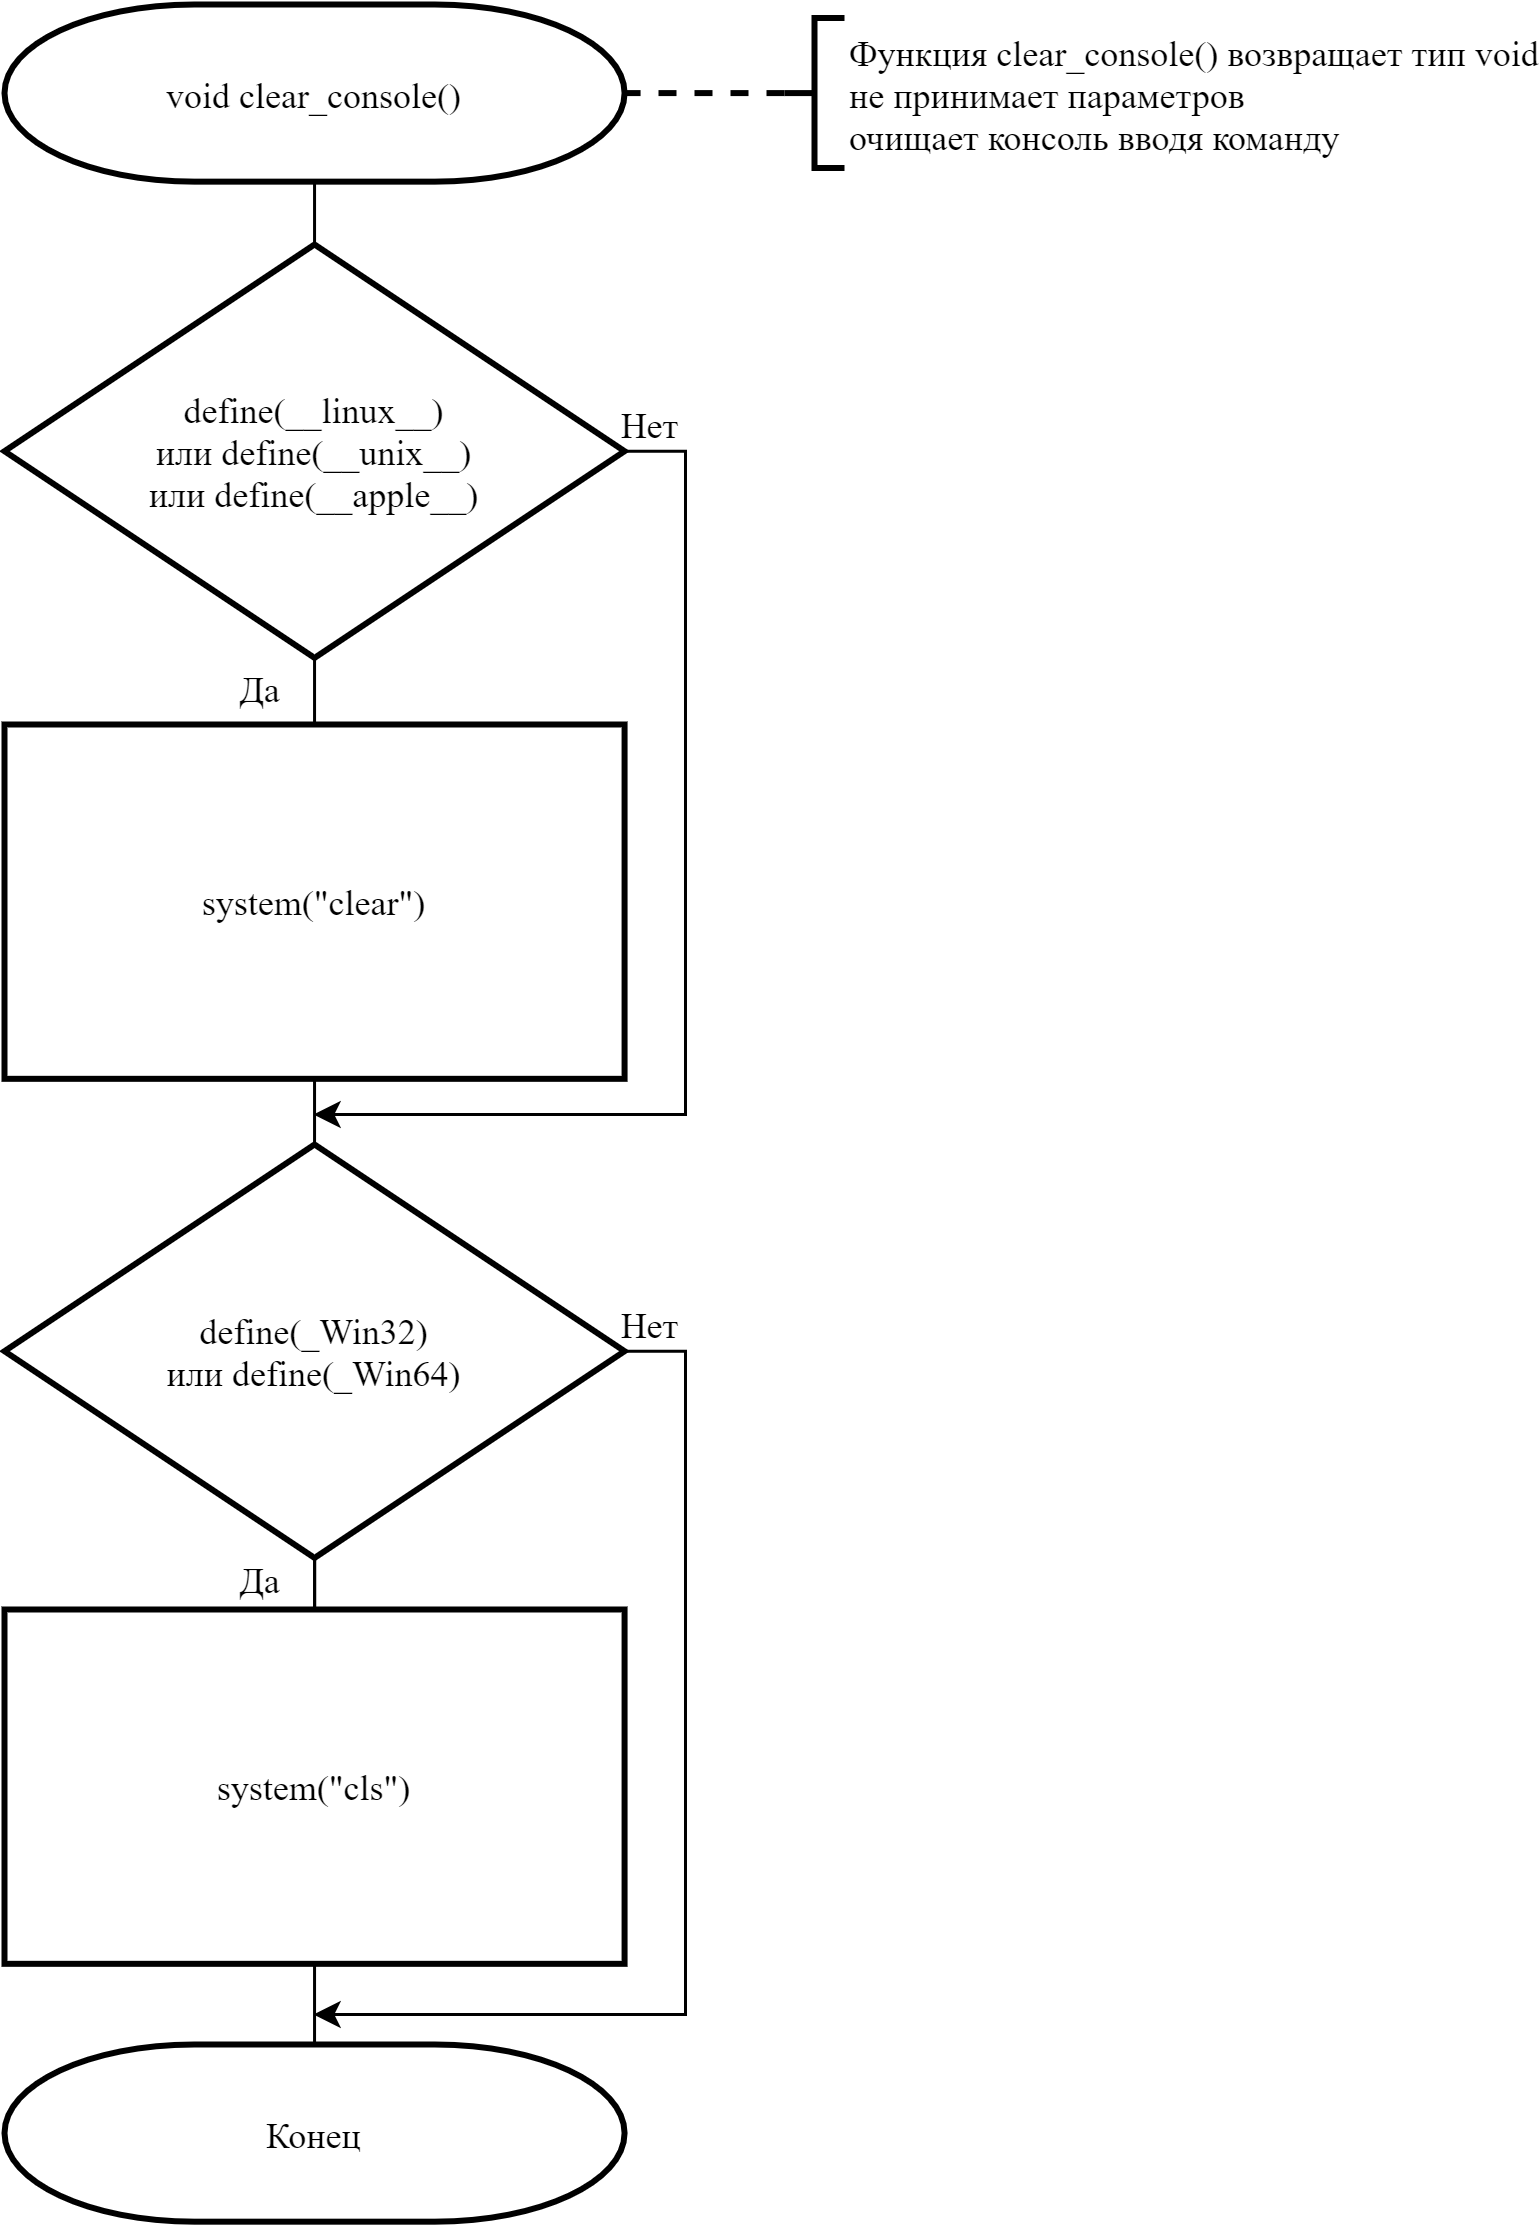
\includegraphics[]{../13/src/my_libs/clearConsole/clearConsole.png}
    }
    \caption{clearConsole()}
    \label{fig:clearConsole}
\end{figure}

\lstinputlisting[
    language=C,
    name=clearConsole.h
]{../13/src/my_libs/clearConsole/clearConsole.h}

\lstinputlisting[
    language=C,
    name=clearConsole.c
]{../13/src/my_libs/clearConsole/clearConsole.c}

\newpage
\subsection{encoding()}

Блок-схема на рисунке \ref{fig:encoding}.

\begin{figure}[h]
    \center{
        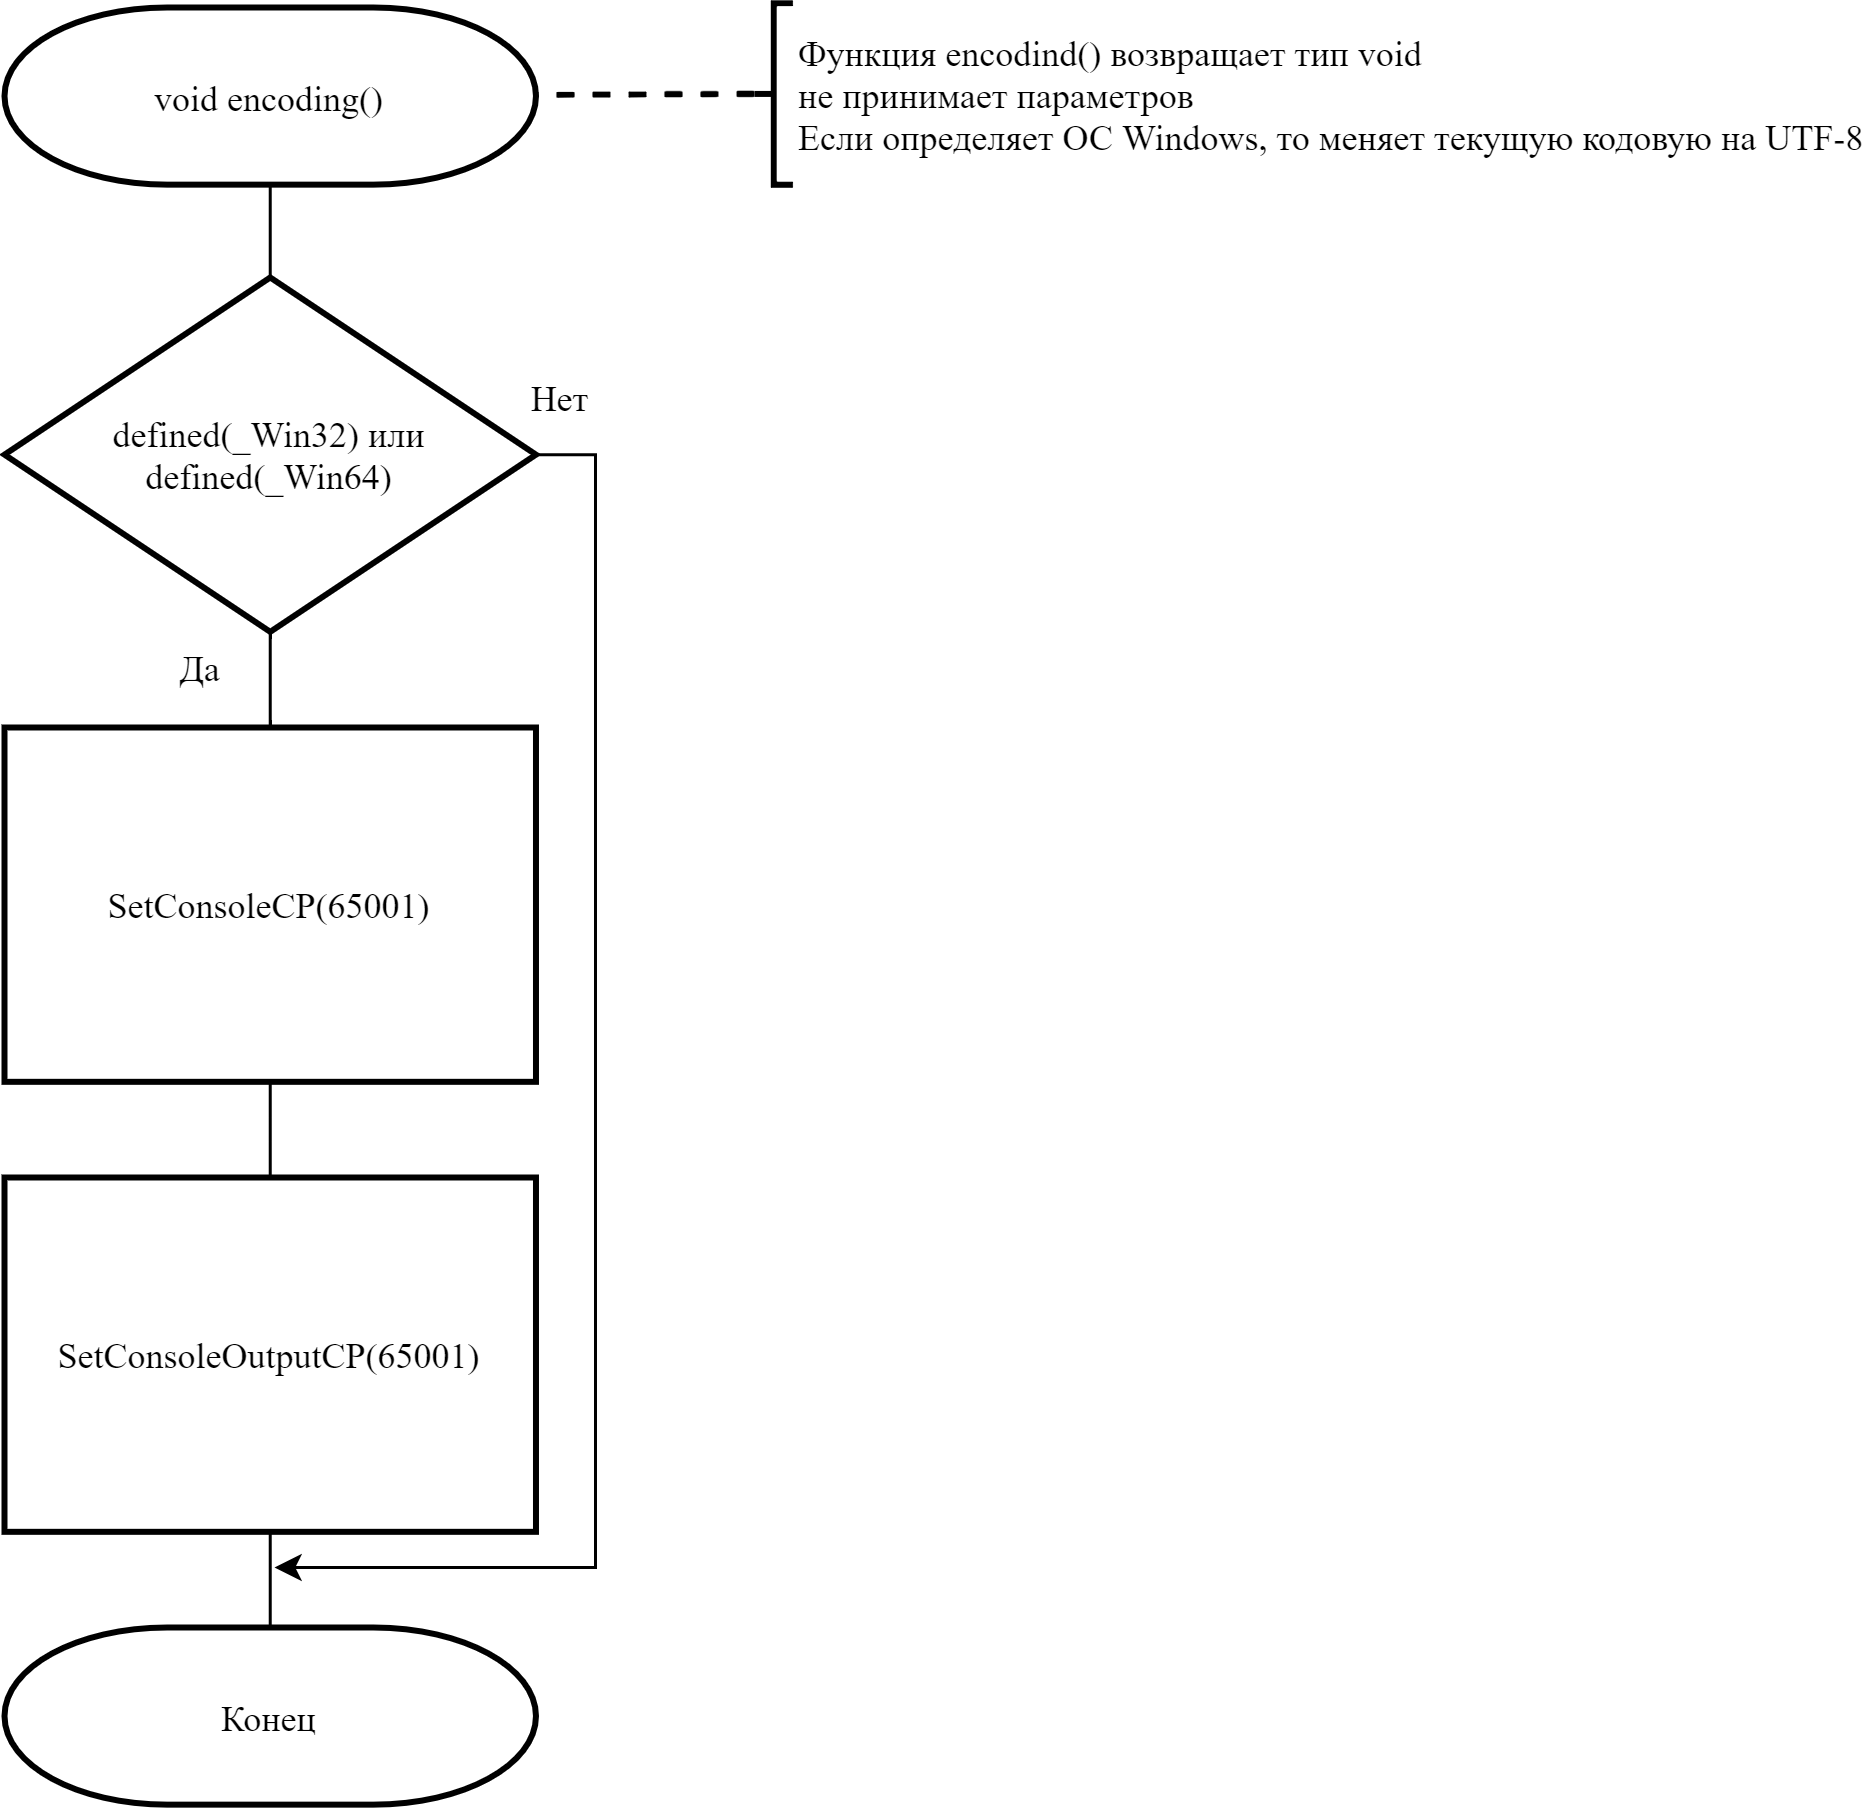
\includegraphics[]{../13/src/my_libs/encoding/encoding.png}
    }
    \caption{encoding()}
    \label{fig:encoding}
\end{figure}

\lstinputlisting[
    language=C,
    name=encoding.h
]{../13/src/my_libs/encoding/encoding.h}

\lstinputlisting[
    language=C,
    name=encoding.c
]{../13/src/my_libs/encoding/encoding.c}

\newpage
\subsection{getch()}

\lstinputlisting[
    language=C,
    name=getch.h
]{../13/src/my_libs/getch/getch.h}

\lstinputlisting[
    language=C,
    name=getch.h
]{../13/src/my_libs/getch/getch.c}

\newpage
\subsection{pause\_console()}

Блок-схема на рисунке \ref{fig:pause_console}.

\begin{figure}[h]
    \center{
        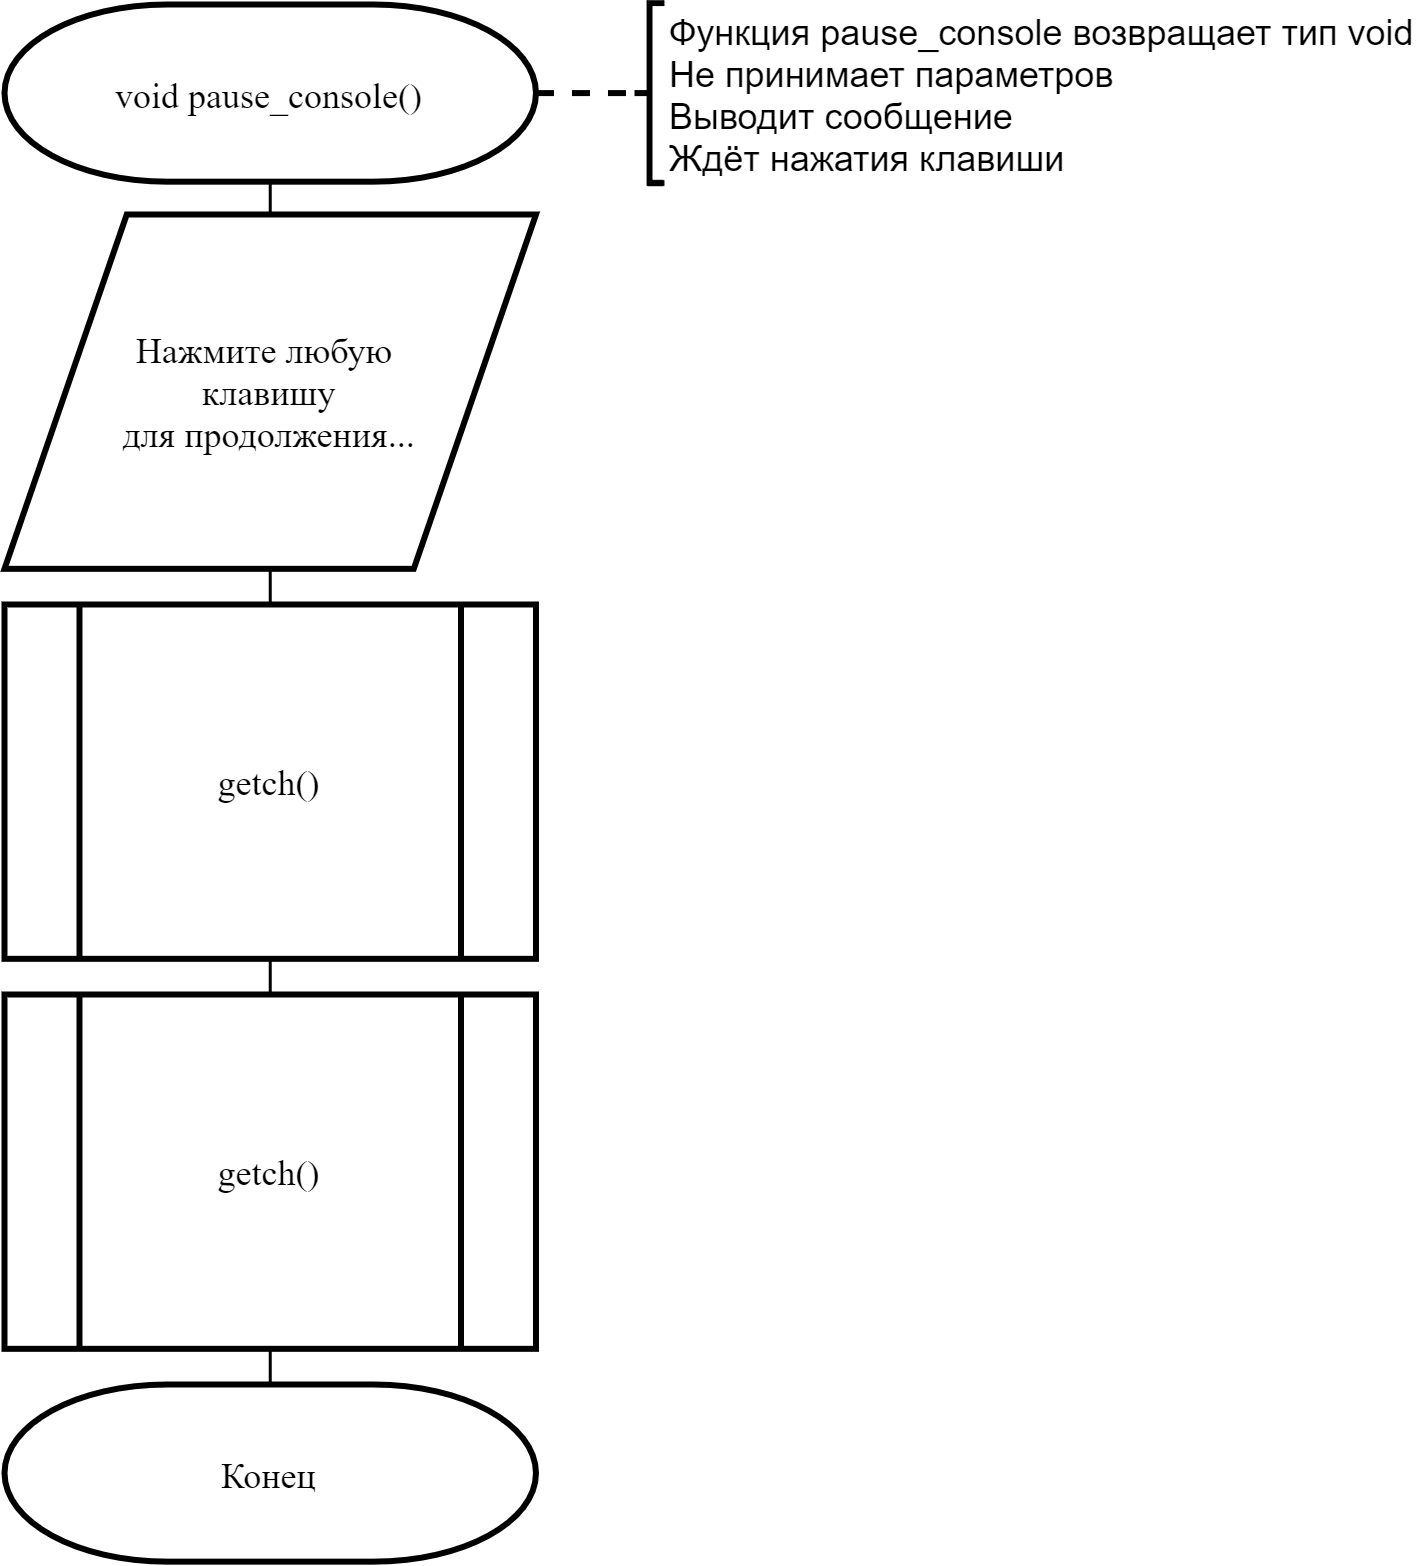
\includegraphics[]{../13/src/my_libs/pause_console/pause_console.png}
    }
    \caption{pause\_console()}
    \label{fig:pause_console}
\end{figure}

\lstinputlisting[
    language=C,
    name=pause\_console.h
]{../13/src/my_libs/pause_console/pause_console.h}

\lstinputlisting[
    language=C,
    name=pause\_console.c
]{../13/src/my_libs/pause_console/pause_console.c}

\newpage

\subsubsection{lab()}

Блок-схема на рисунке \ref{fig:lab}.

\begin{figure}[h]
    \center{
        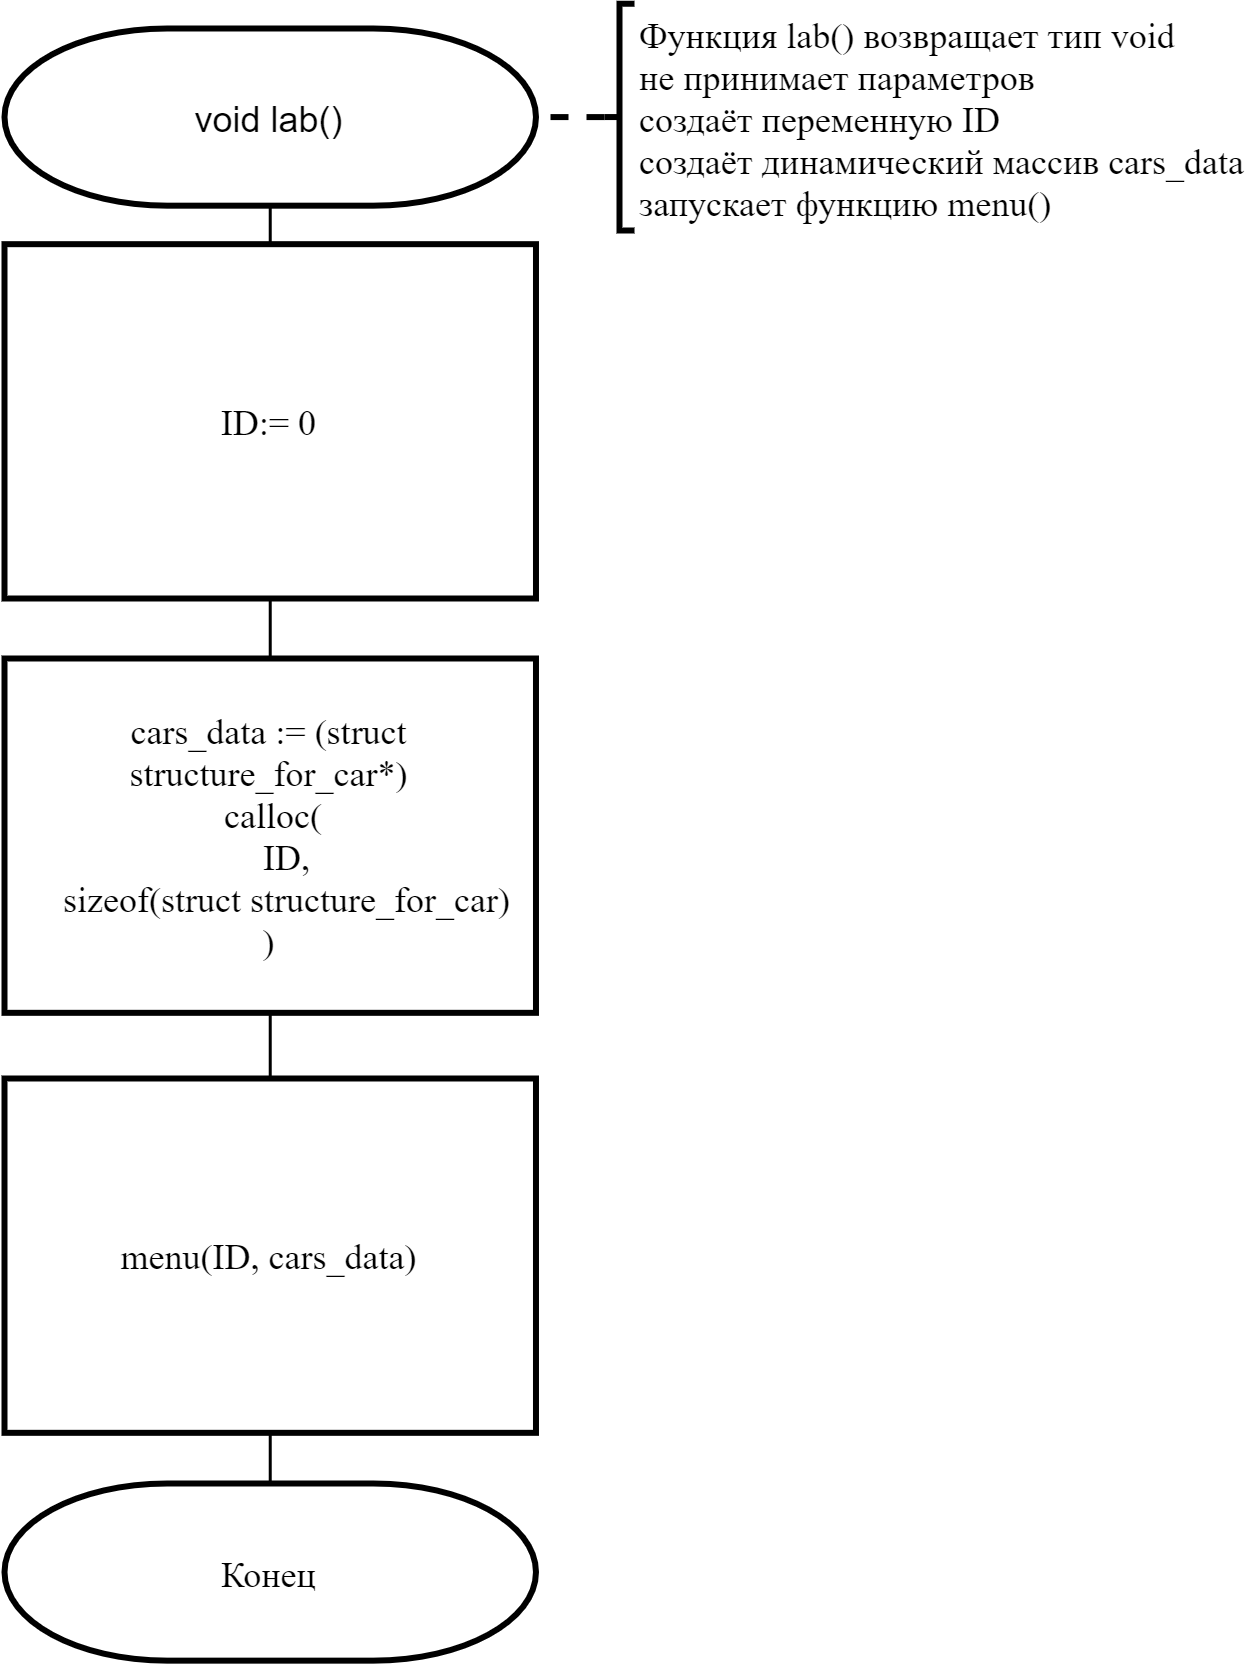
\includegraphics[]{../13/src/lab/lab.png}
    }
    \caption{lab()}
    \label{fig:lab}
\end{figure}

\lstinputlisting[
    language=C,
    name=lab.h
]{../13/src/lab/lab.h}

\lstinputlisting[
    language=C,
    name=lab.c
]{../13/src/lab/lab.c}

\newpage
\subsubsection{menu()}

Блок-схема на рисунке \ref{fig:menu}.

\begin{figure}[p]
    \center{
        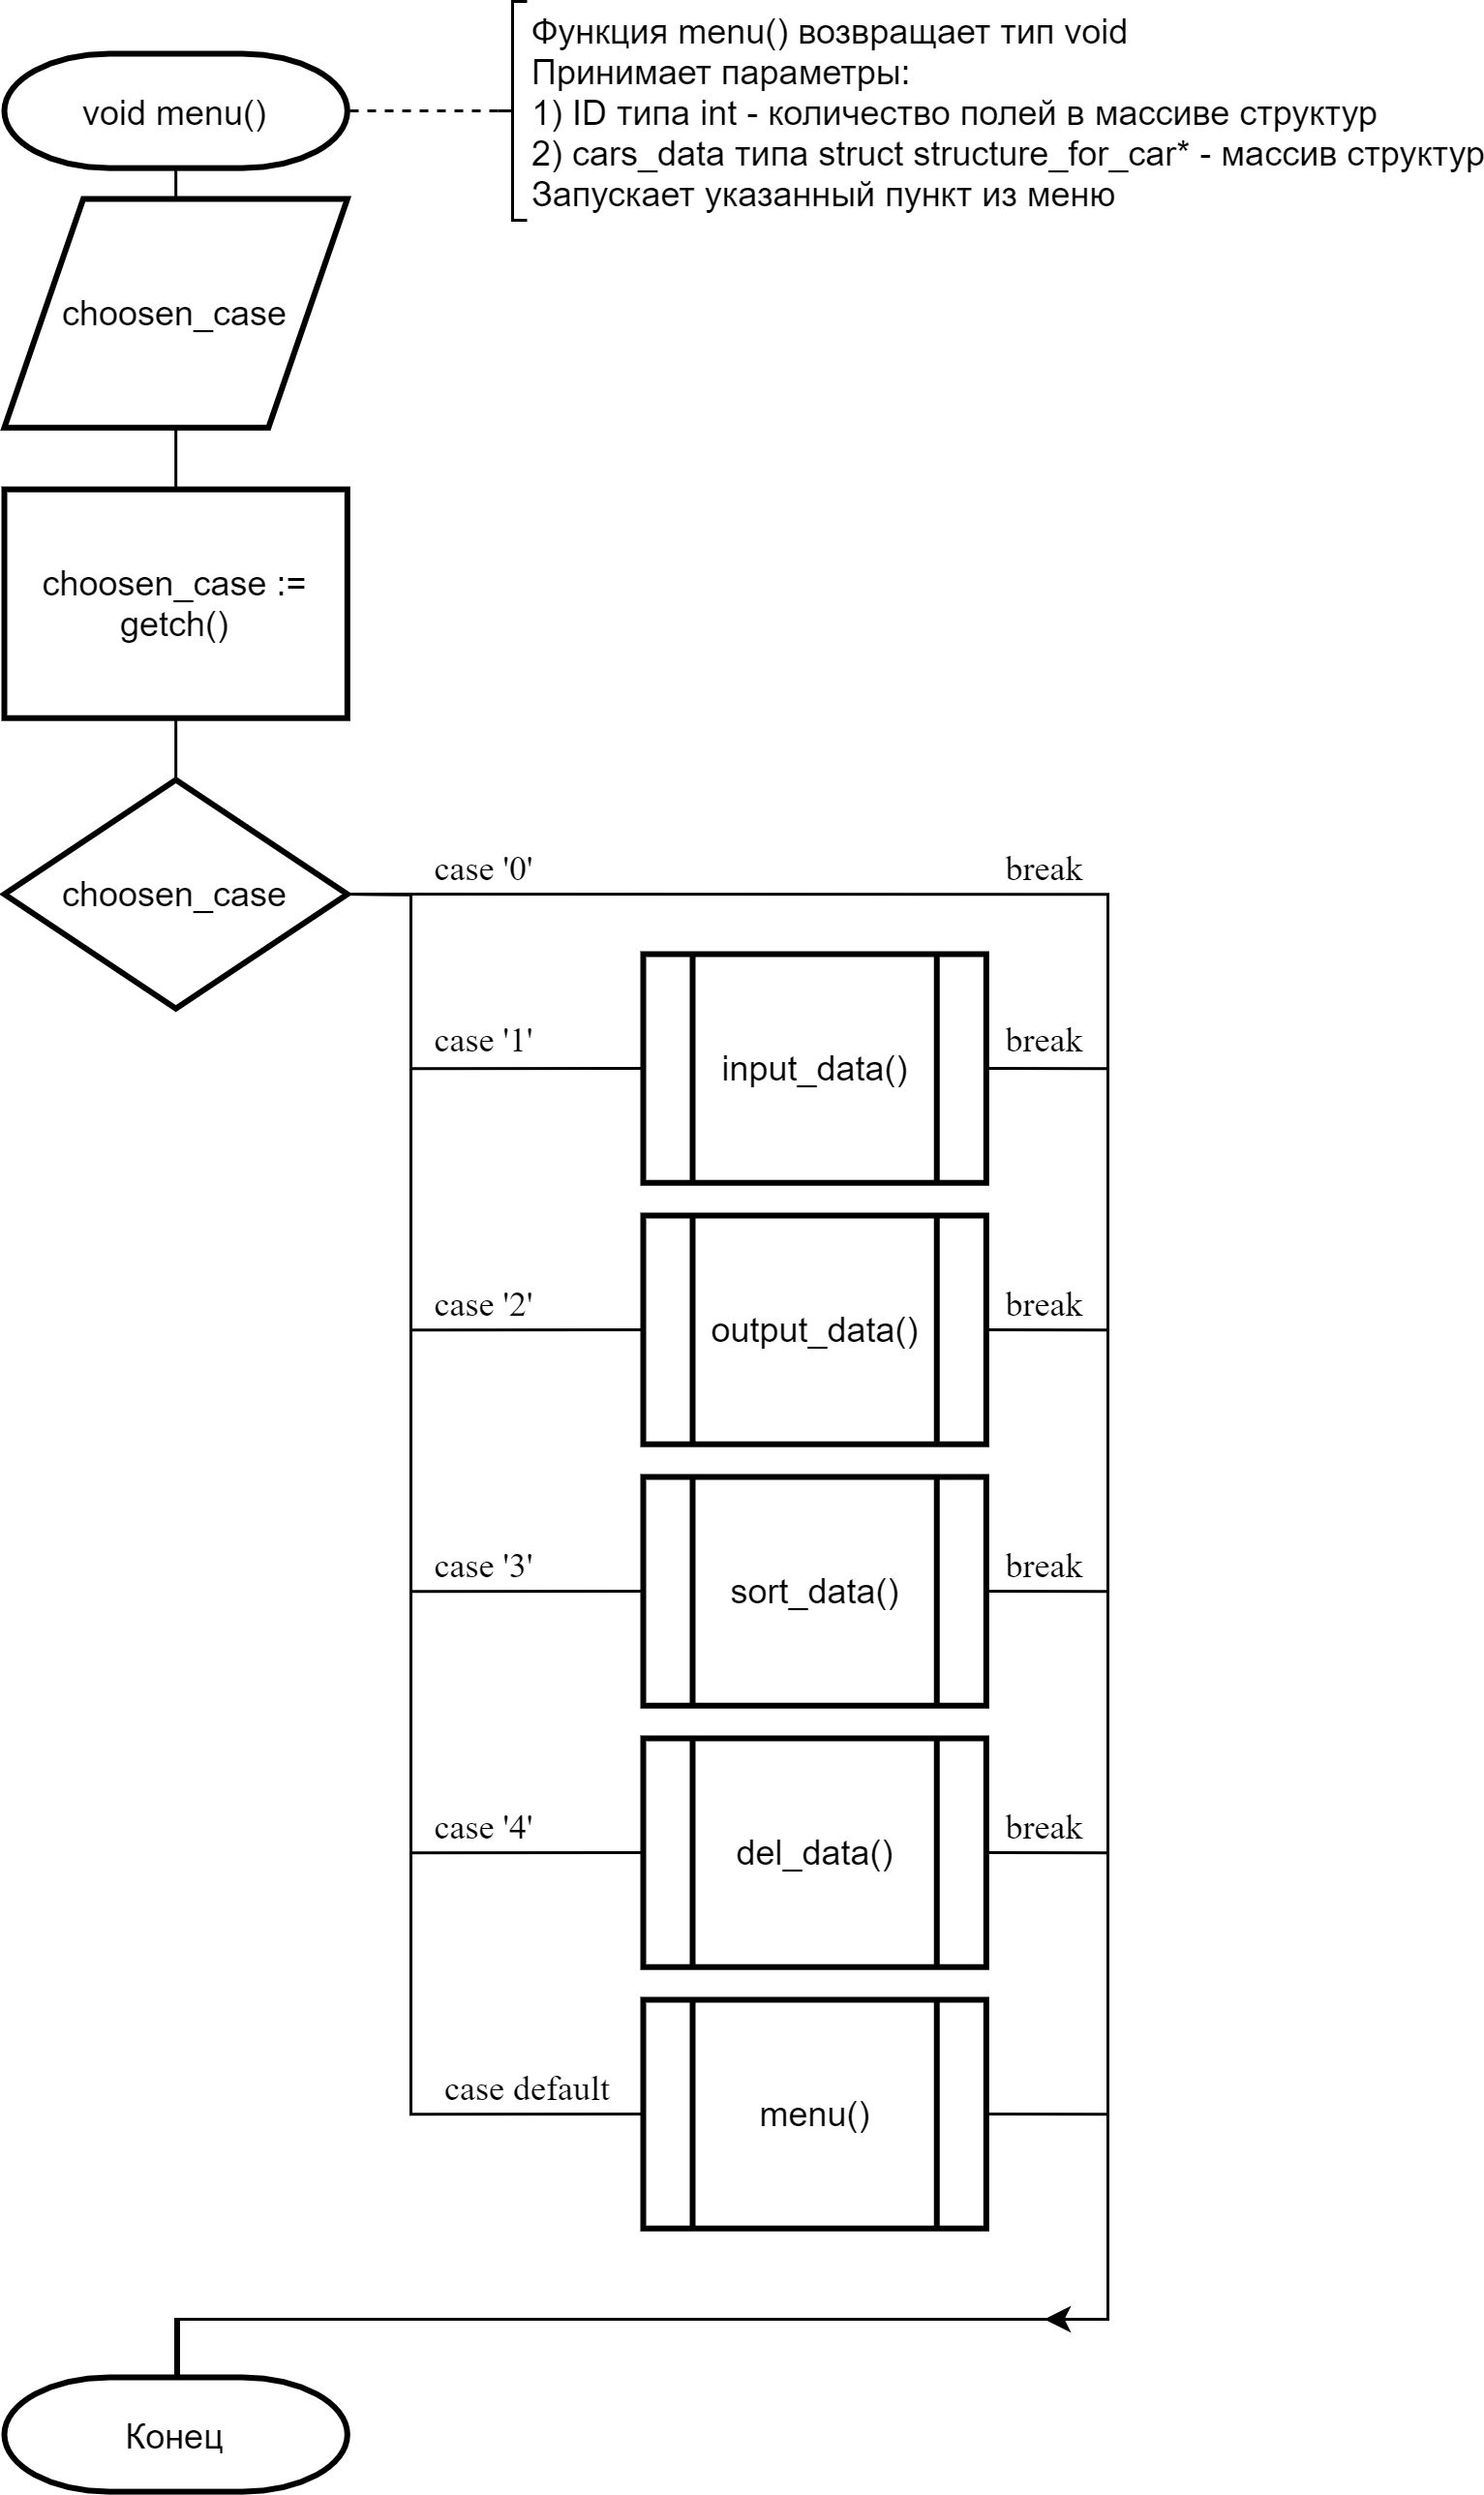
\includegraphics[]{../13/src/lab/menu/menu.png}
    }
    \caption{menu()}
    \label{fig:menu}
\end{figure}

\lstinputlisting[
    language=C,
    name=menu.h
]{../13/src/lab/menu/menu.h}

\lstinputlisting[
    language=C,
    name=menu.c
]{../13/src/lab/menu/menu.c}

\newpage
\subsection{del\_data()}

Блок-схема на рисунке \ref{fig:del_data}.

\begin{figure}[p]
    \center{
        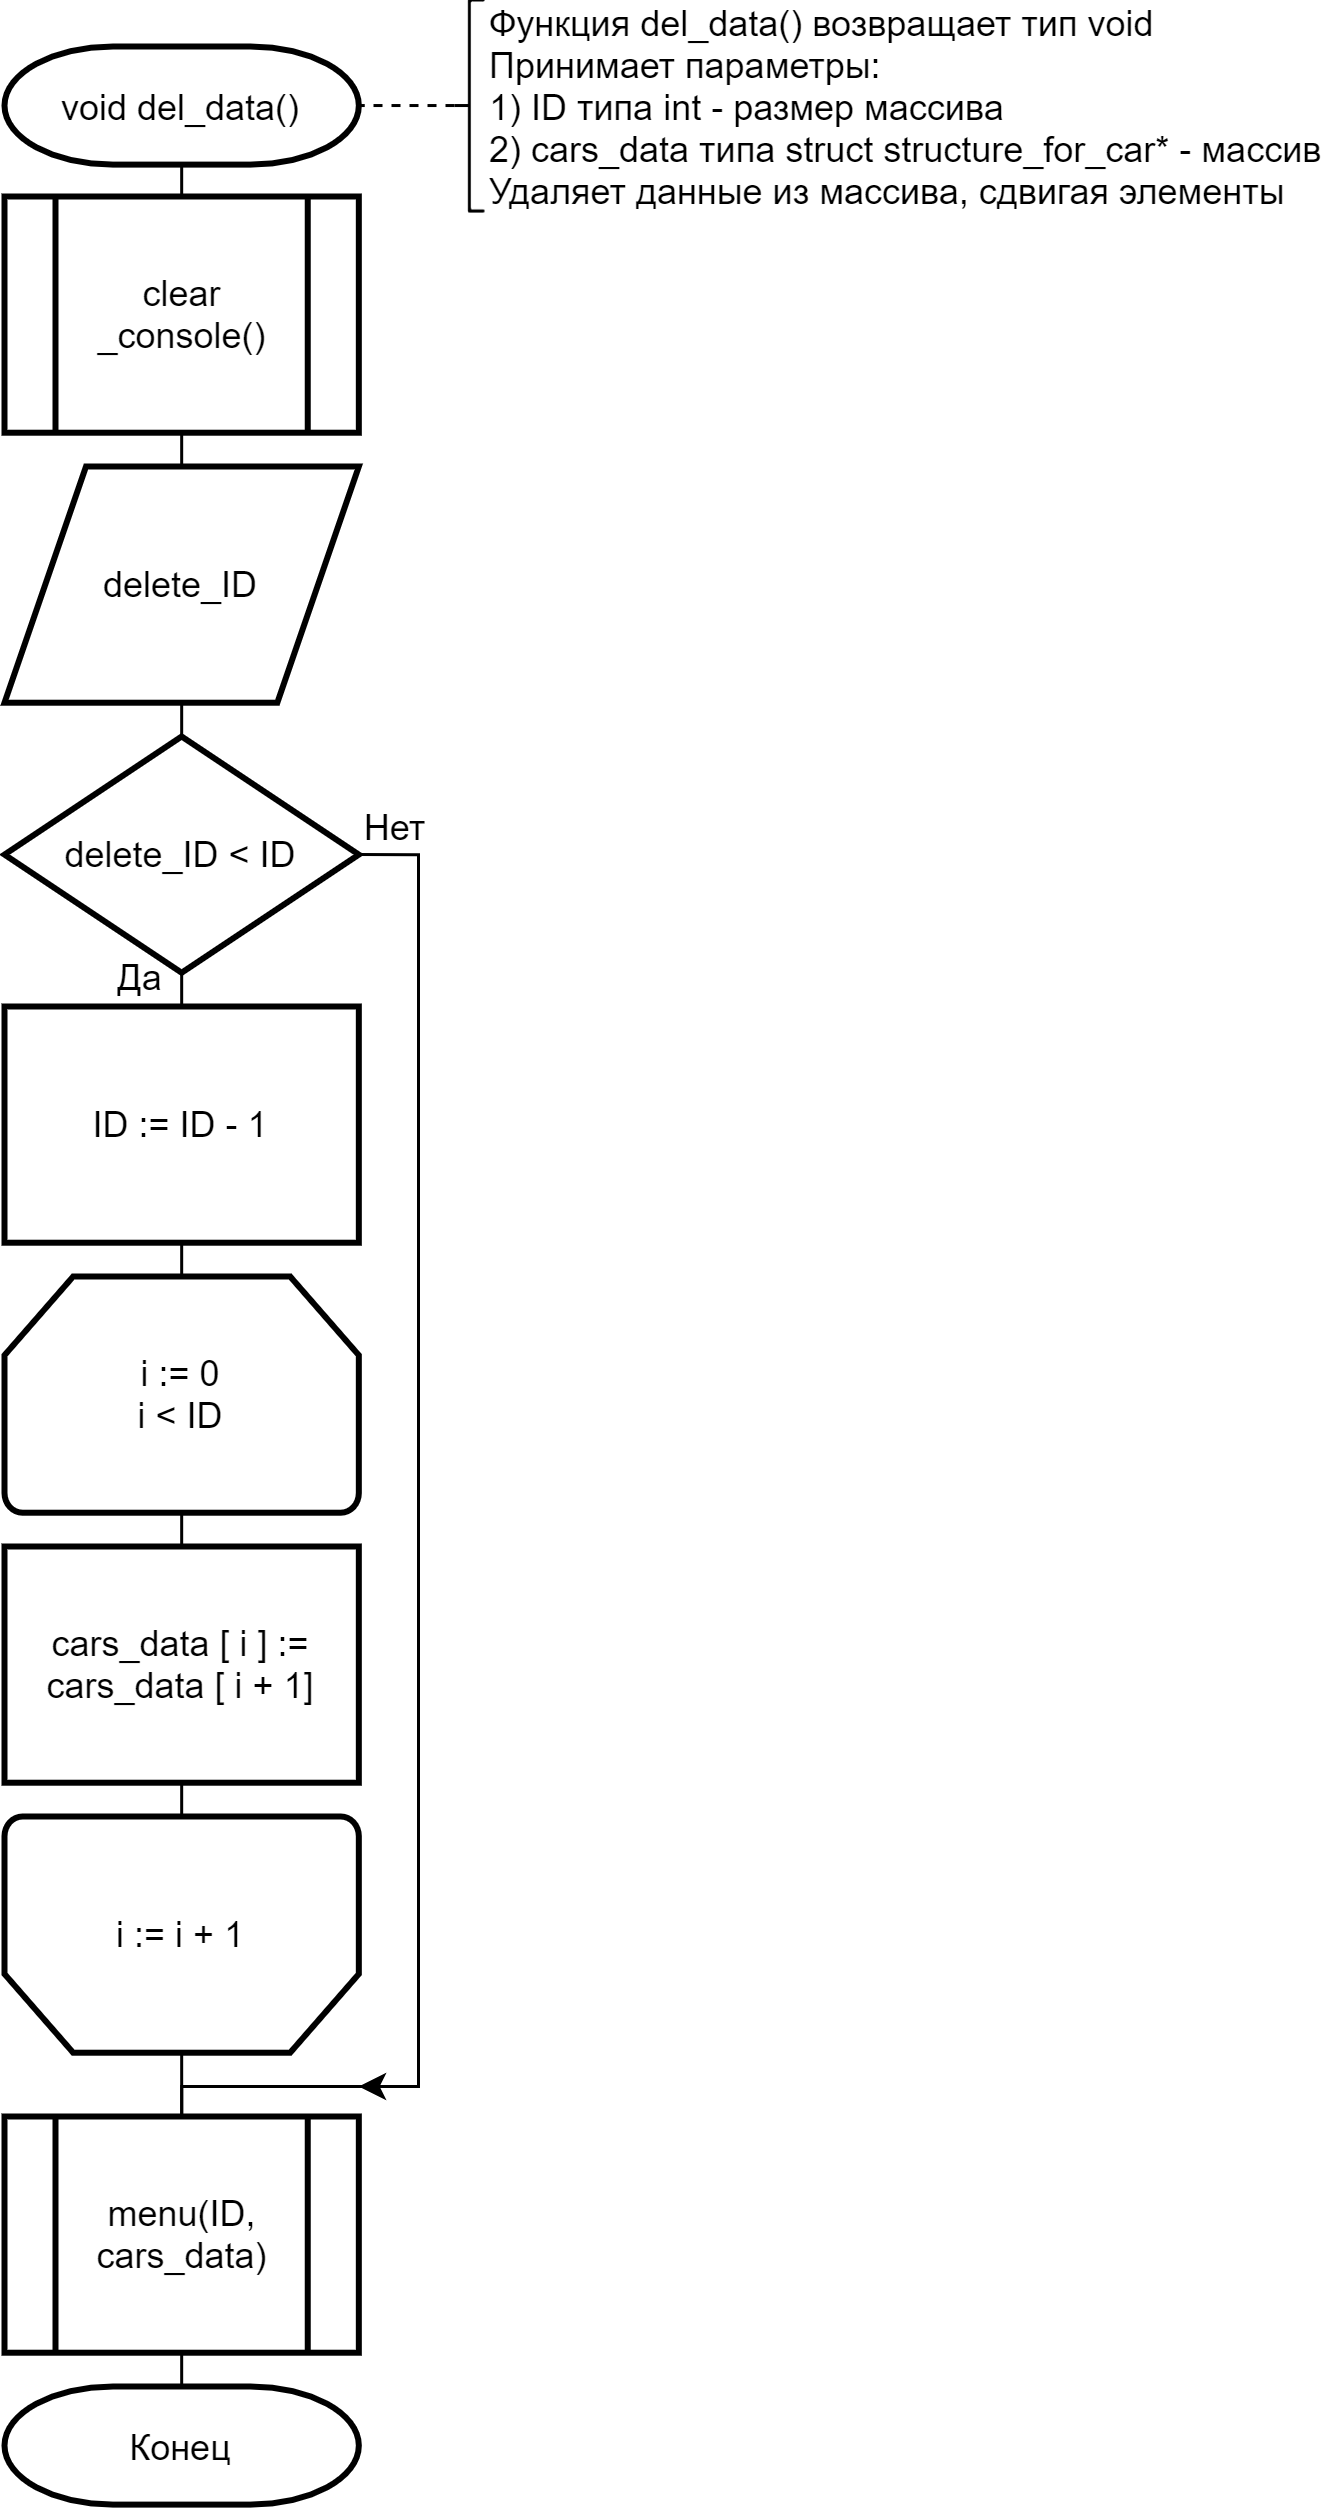
\includegraphics[]{../13/src/lab/menu/del_data/del_data.png}
    }
    \caption{del\_data()}
    \label{fig:del_data}
\end{figure}

\lstinputlisting[
    language=C,
    name=del\_data.h
]{../13/src/lab/menu/del_data/del_data.h}

\lstinputlisting[
    language=C,
    name=del\_data.c
]{../13/src/lab/menu/del_data/del_data.c}

\newpage
\subsubsection{input\_data()}

Блок-схема на рисунке \ref{fig:input_data}.

\begin{figure}[p]
    \center{
        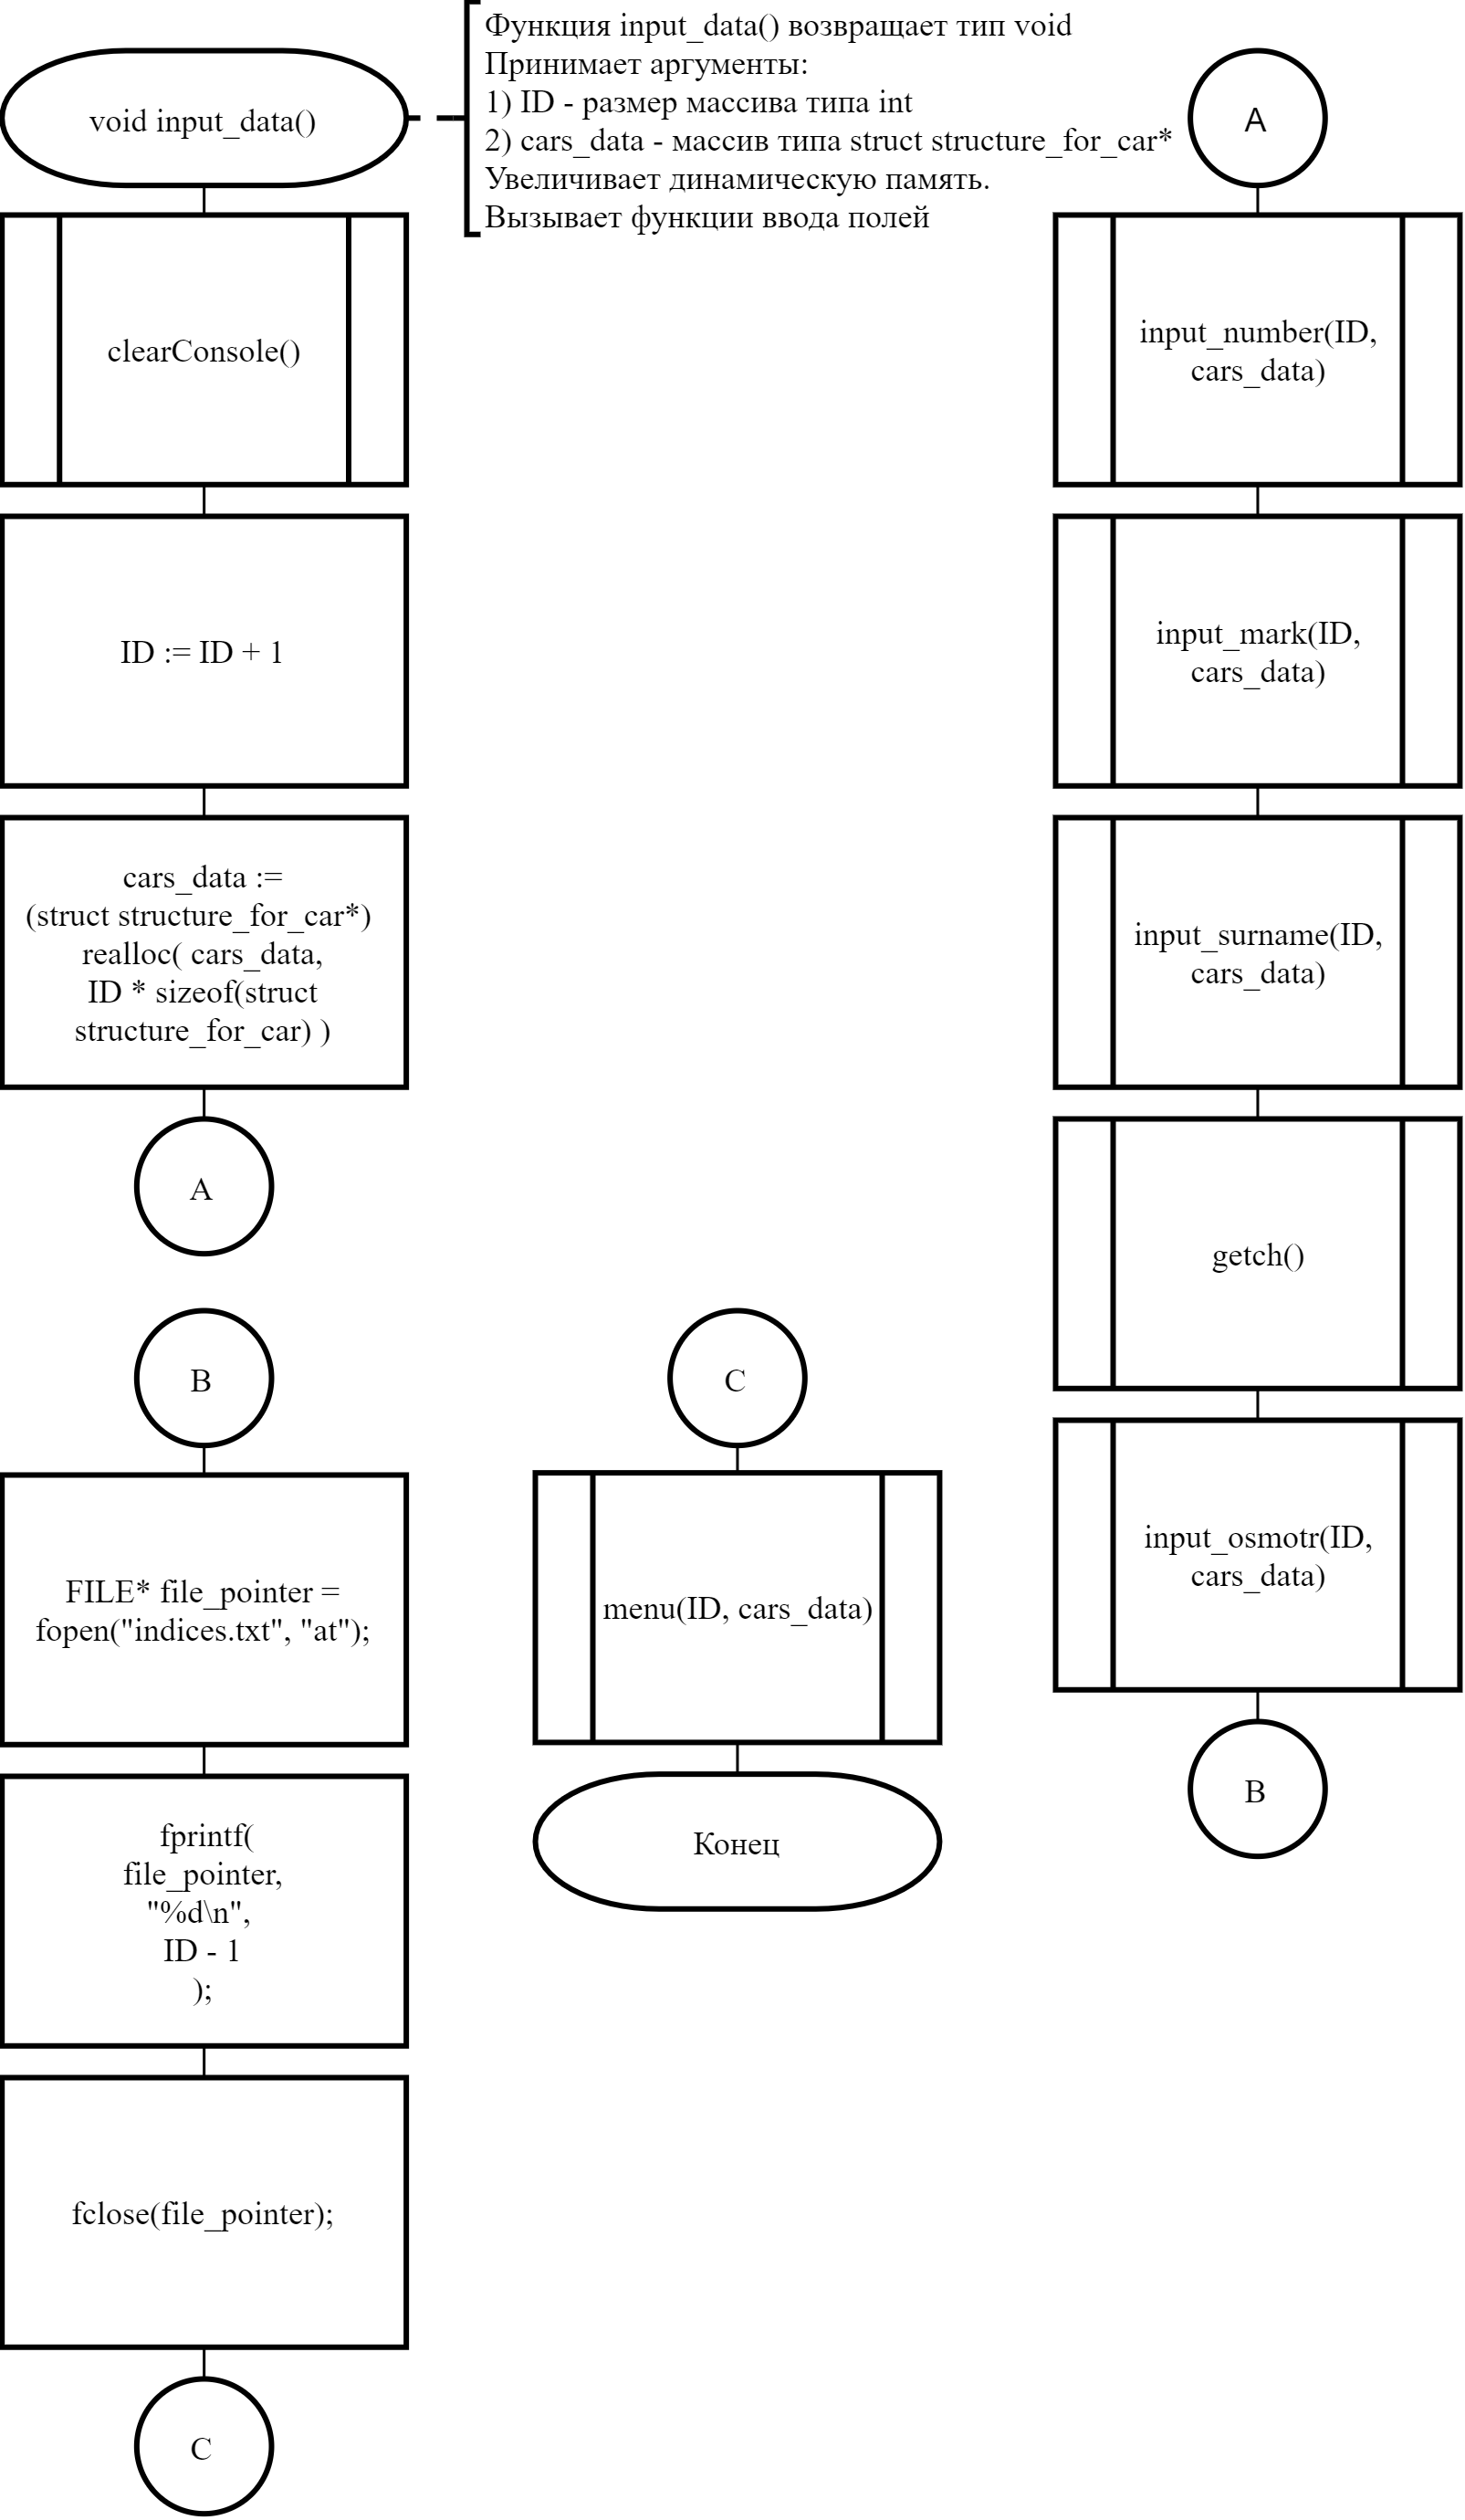
\includegraphics[width=16cm]{../13/src/lab/menu/input_data/input_data.png}
    }
    \caption{input\_data()}
    \label{fig:input_data}
\end{figure}

\lstinputlisting[
    language=C,
    name=input\_data.h
]{../13/src/lab/menu/input_data/input_data.h}

\lstinputlisting[
    language=C,
    name=input\_data.c
]{../13/src/lab/menu/input_data/input_data.c}

\newpage
\subsection{out\_data()}

Блок-схема на рисунке \ref{fig:out_data}.

\begin{figure}[p]
    \center{
        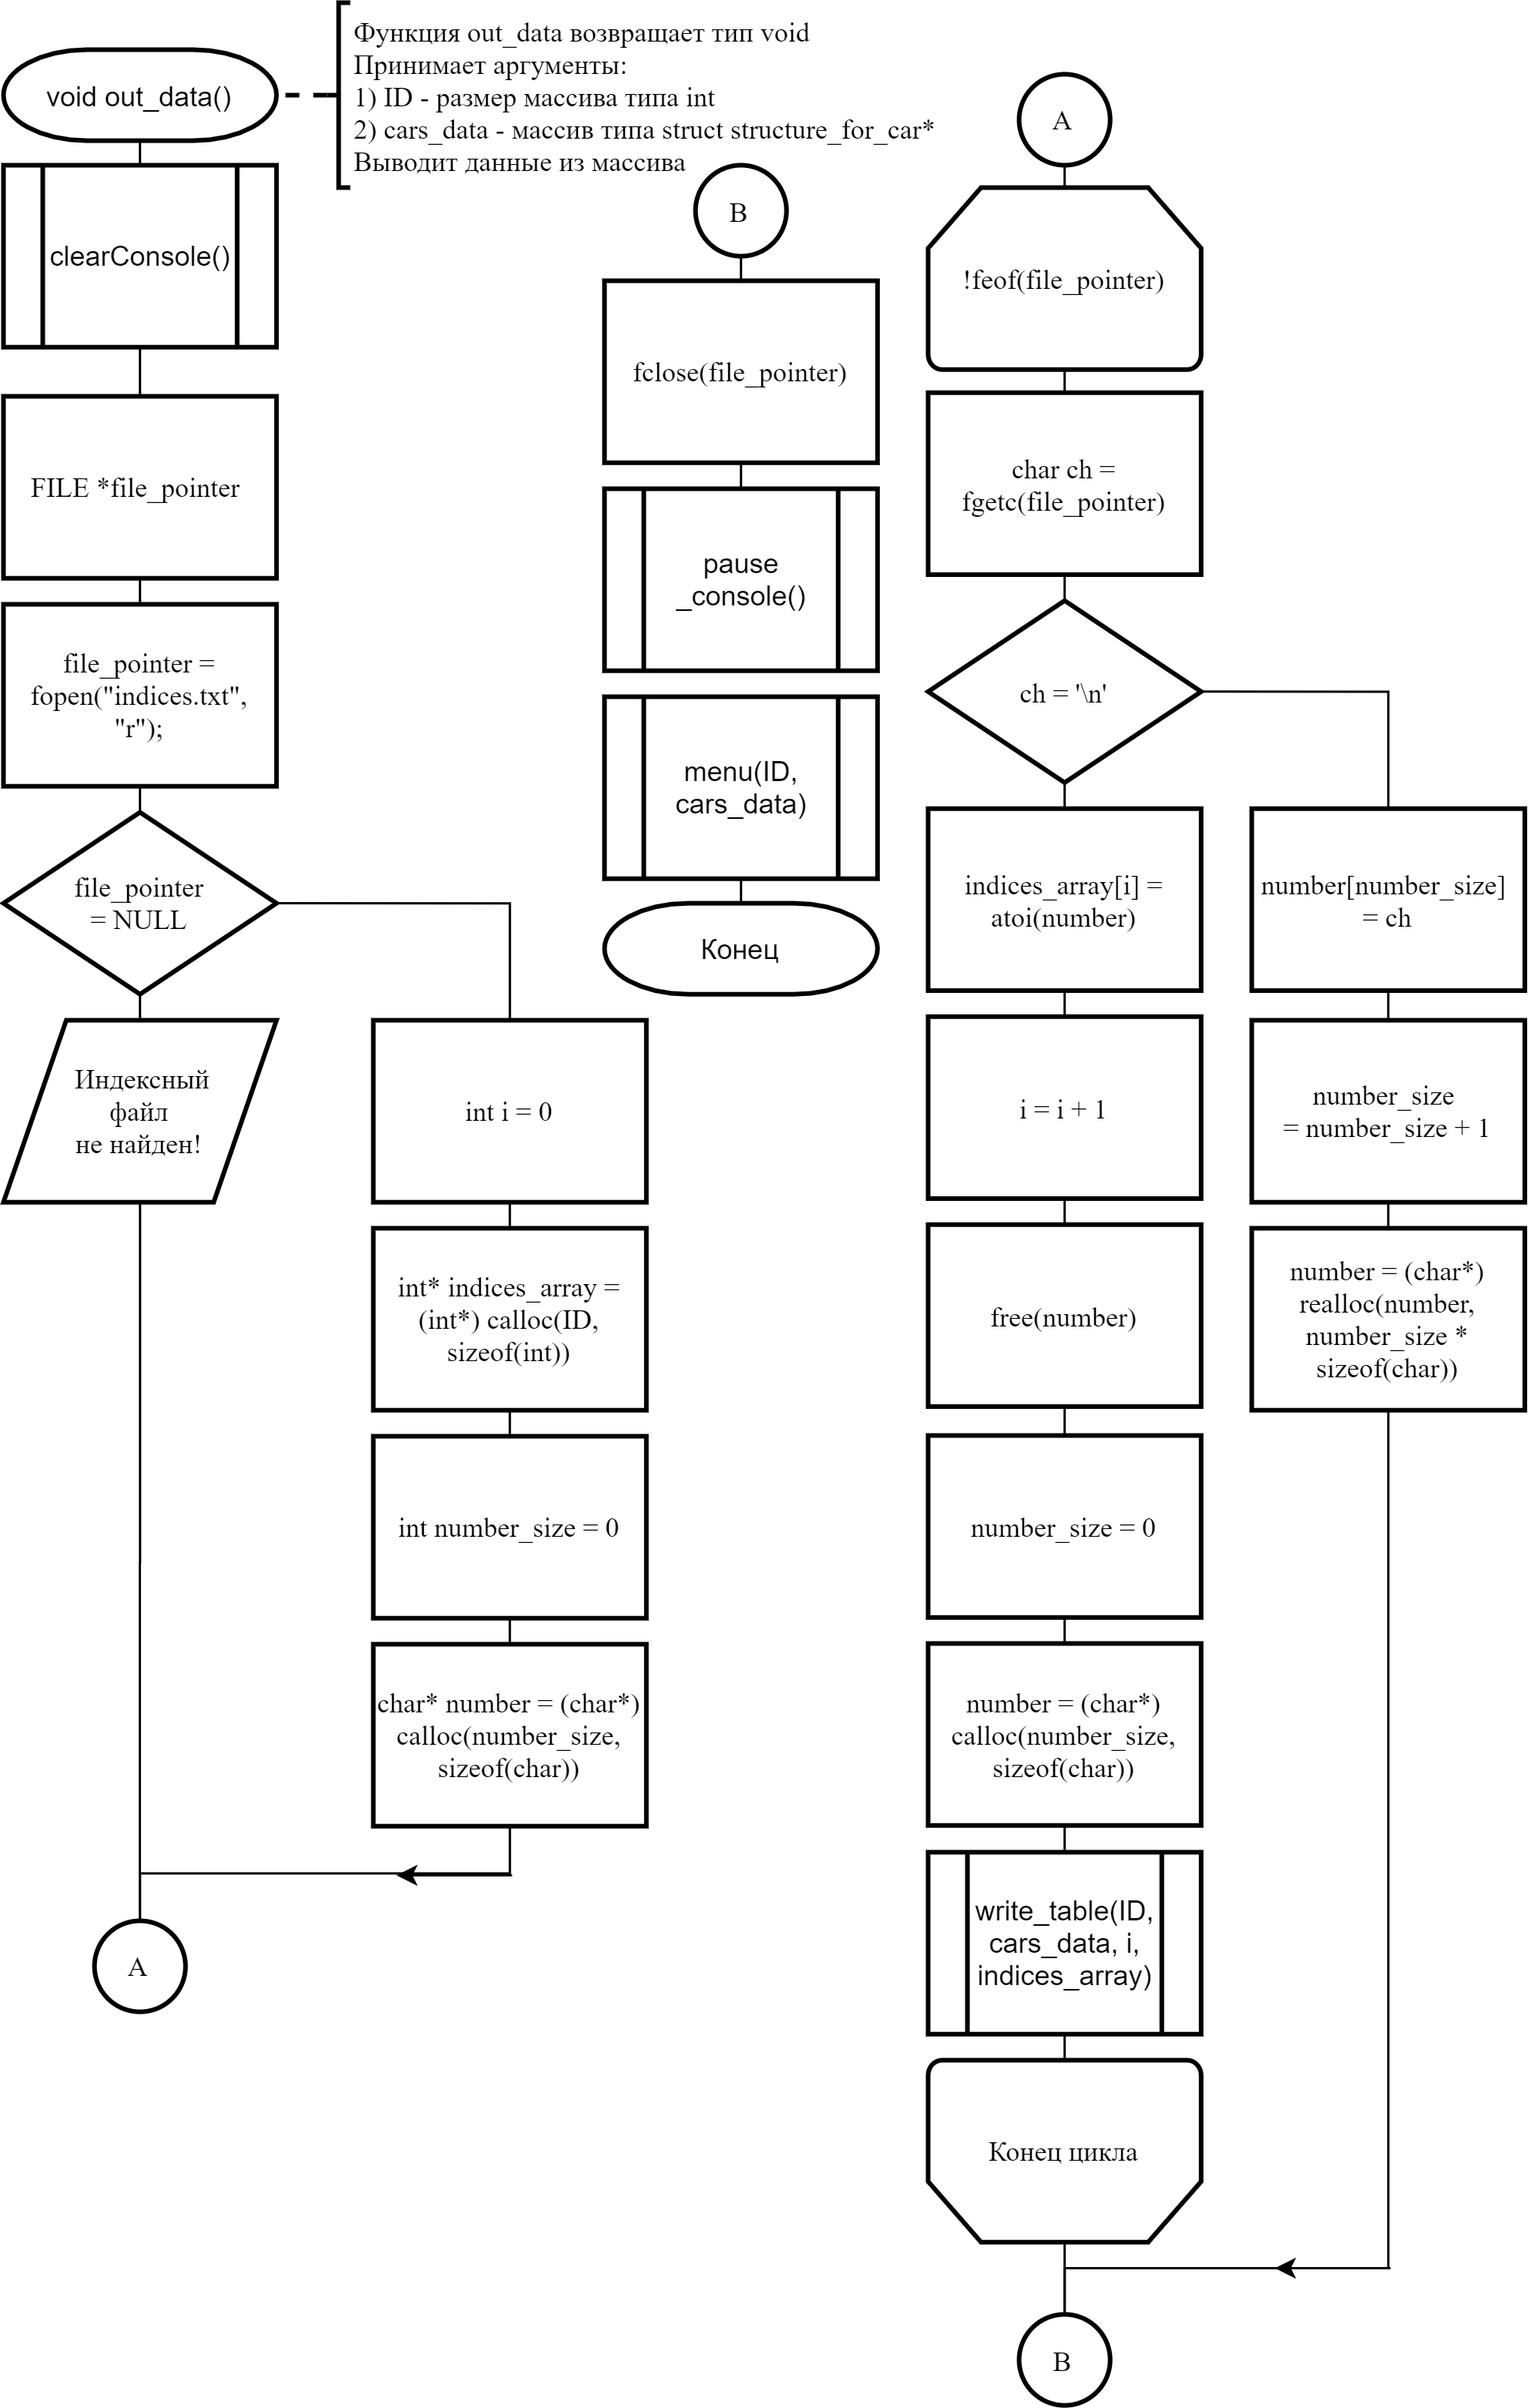
\includegraphics[]{../13/src/lab/menu/out_data/out_data.png}
    }
    \caption{out\_data()}
    \label{fig:out_data}
\end{figure}

\lstinputlisting[
    language=C,
    name=out\_data.h
]{../13/src/lab/menu/out_data/out_data.h}

\lstinputlisting[
    language=C,
    name=out\_data.c
]{../13/src/lab/menu/out_data/out_data.c}

\newpage
\subsubsection{sort\_data()}

Блок-схема на рисунке \ref{fig:sort_data}.

\begin{figure}[p]
    \center{
        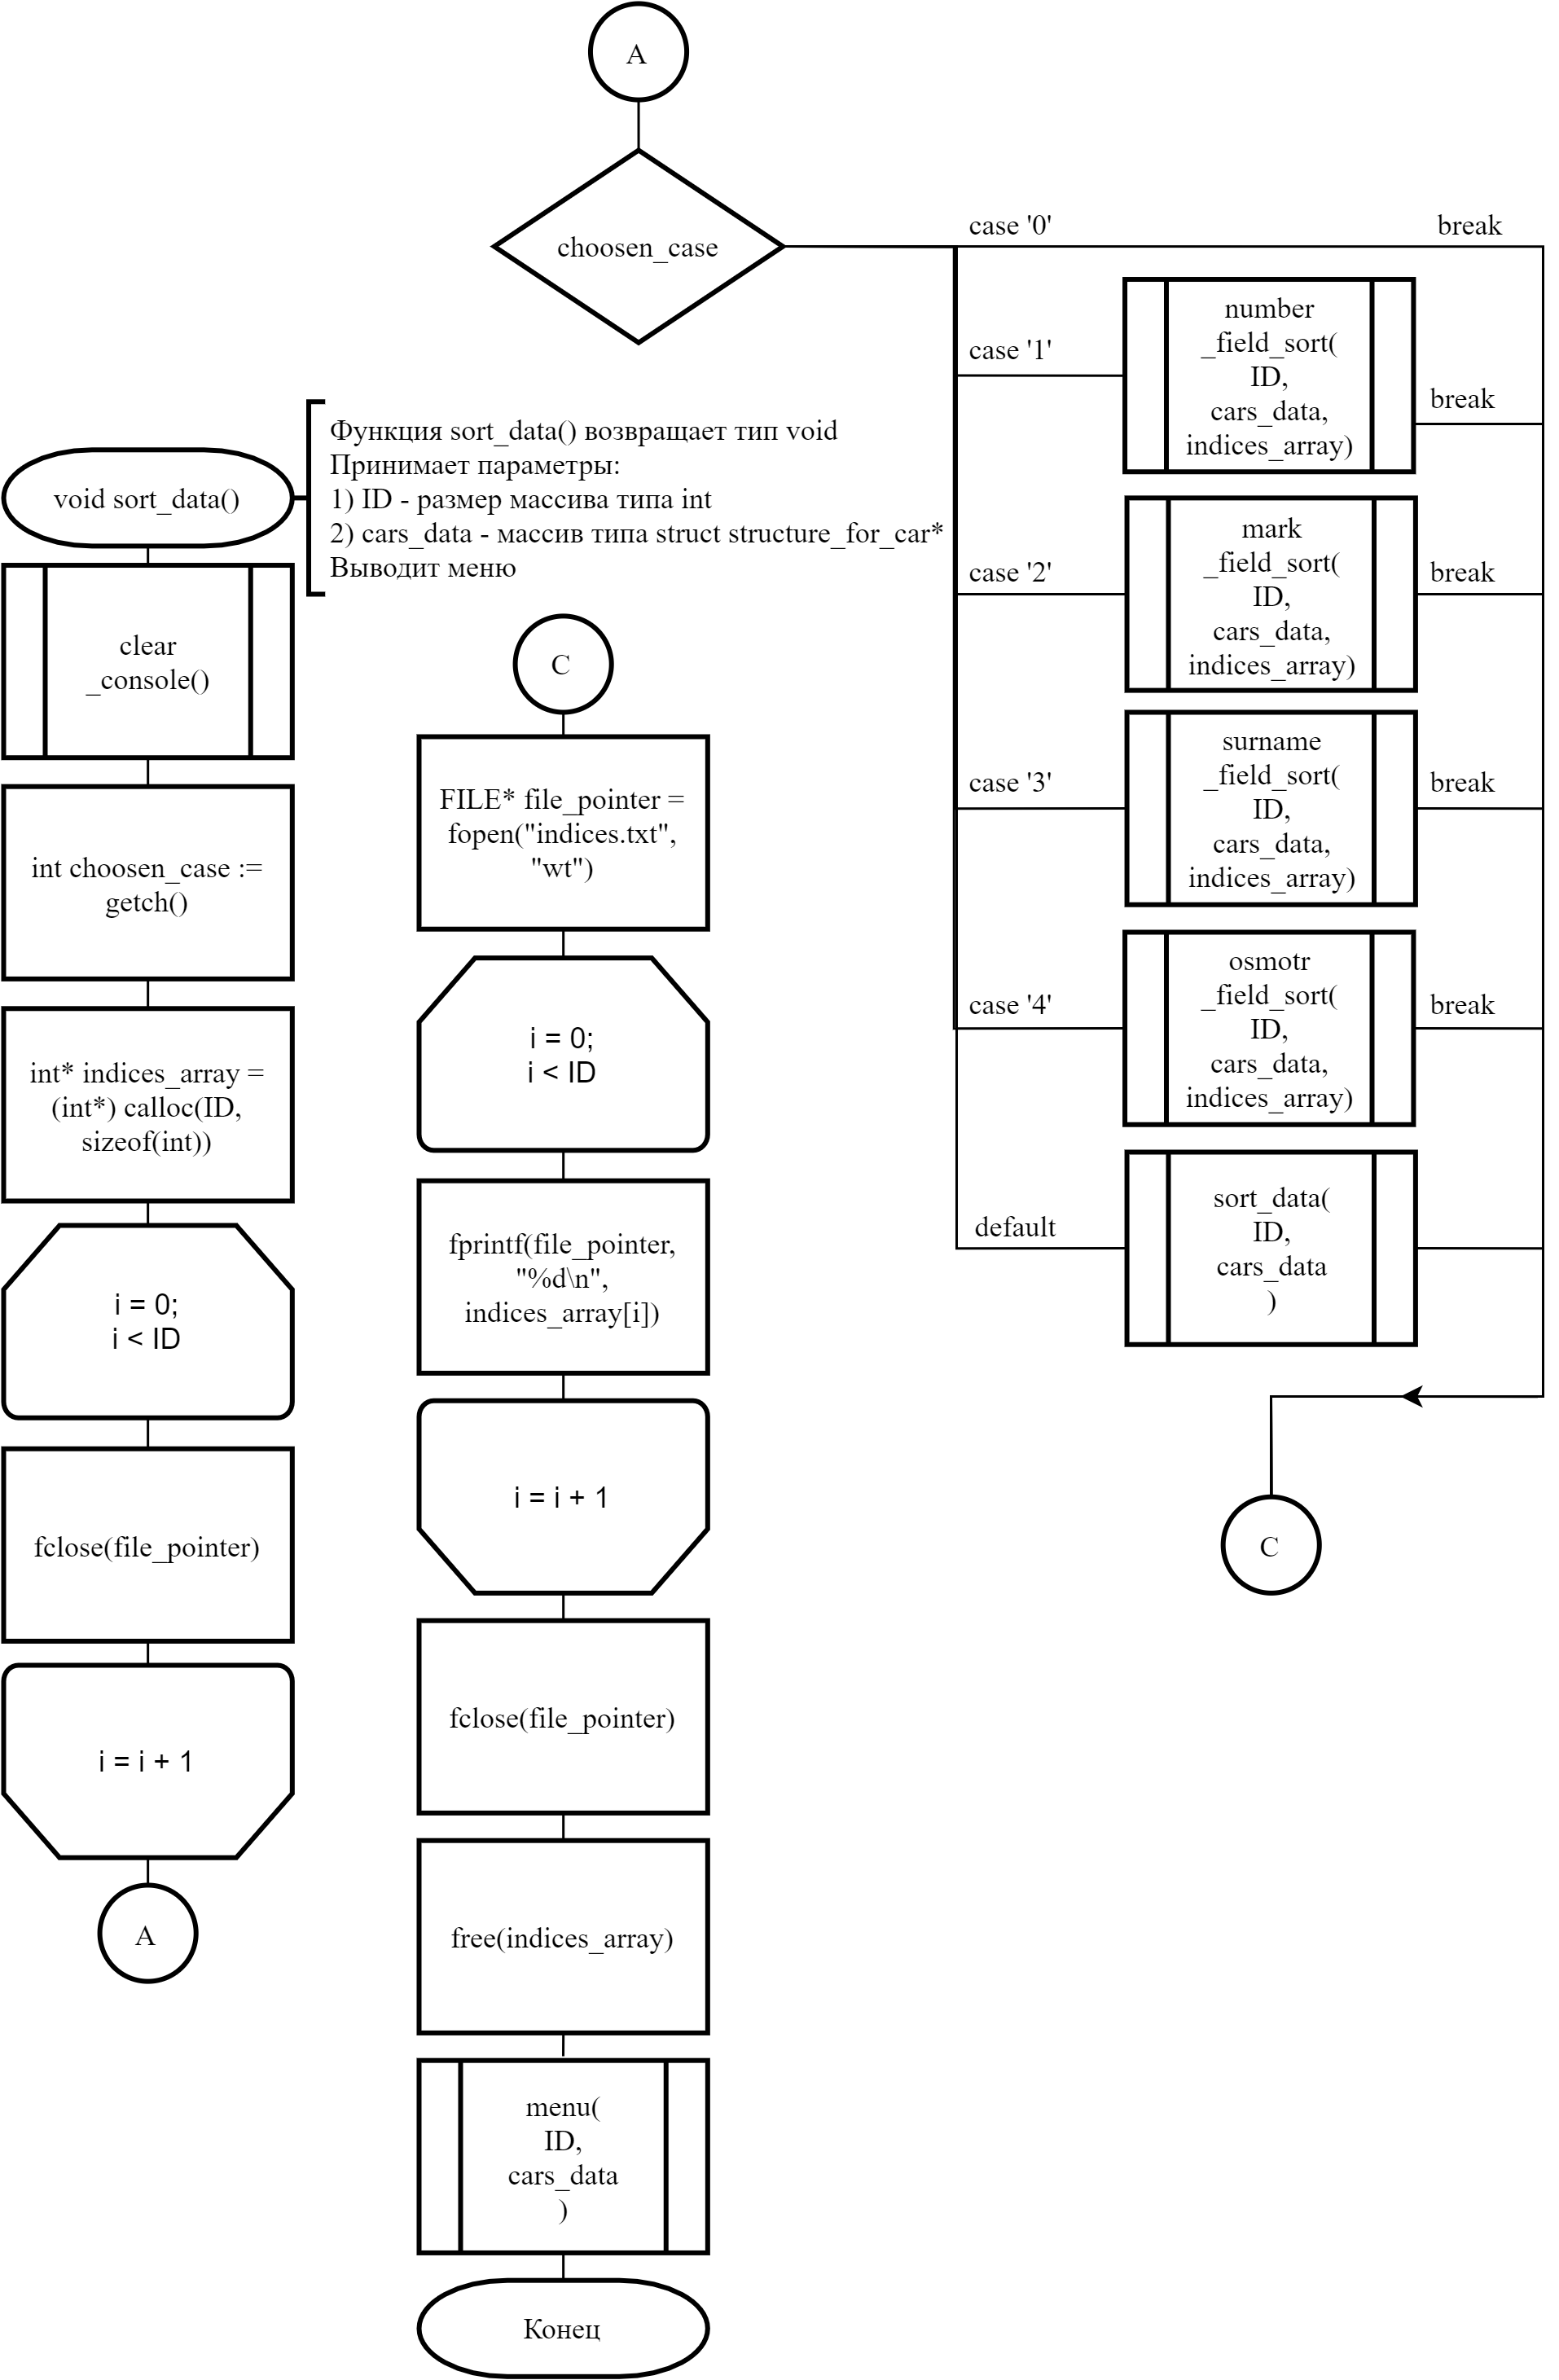
\includegraphics[]{../13/src/lab/menu/sort_data/sort_data.png}
    }
    \caption{sort\_data()}
    \label{fig:sort_data}
\end{figure}

\lstinputlisting[
    language=C,
    name=sort\_data.h
]{../13/src/lab/menu/sort_data/sort_data.h}

\lstinputlisting[
    language=C,
    name=sort\_data.c
]{../13/src/lab/menu/sort_data/sort_data.c}

\newpage

\subsection{sort\_data\_by\_mark\_field()}

Блок-схема на рисунке \ref{fig:sort_data_by_mark_field}.

\begin{figure}[p]
    \center{
        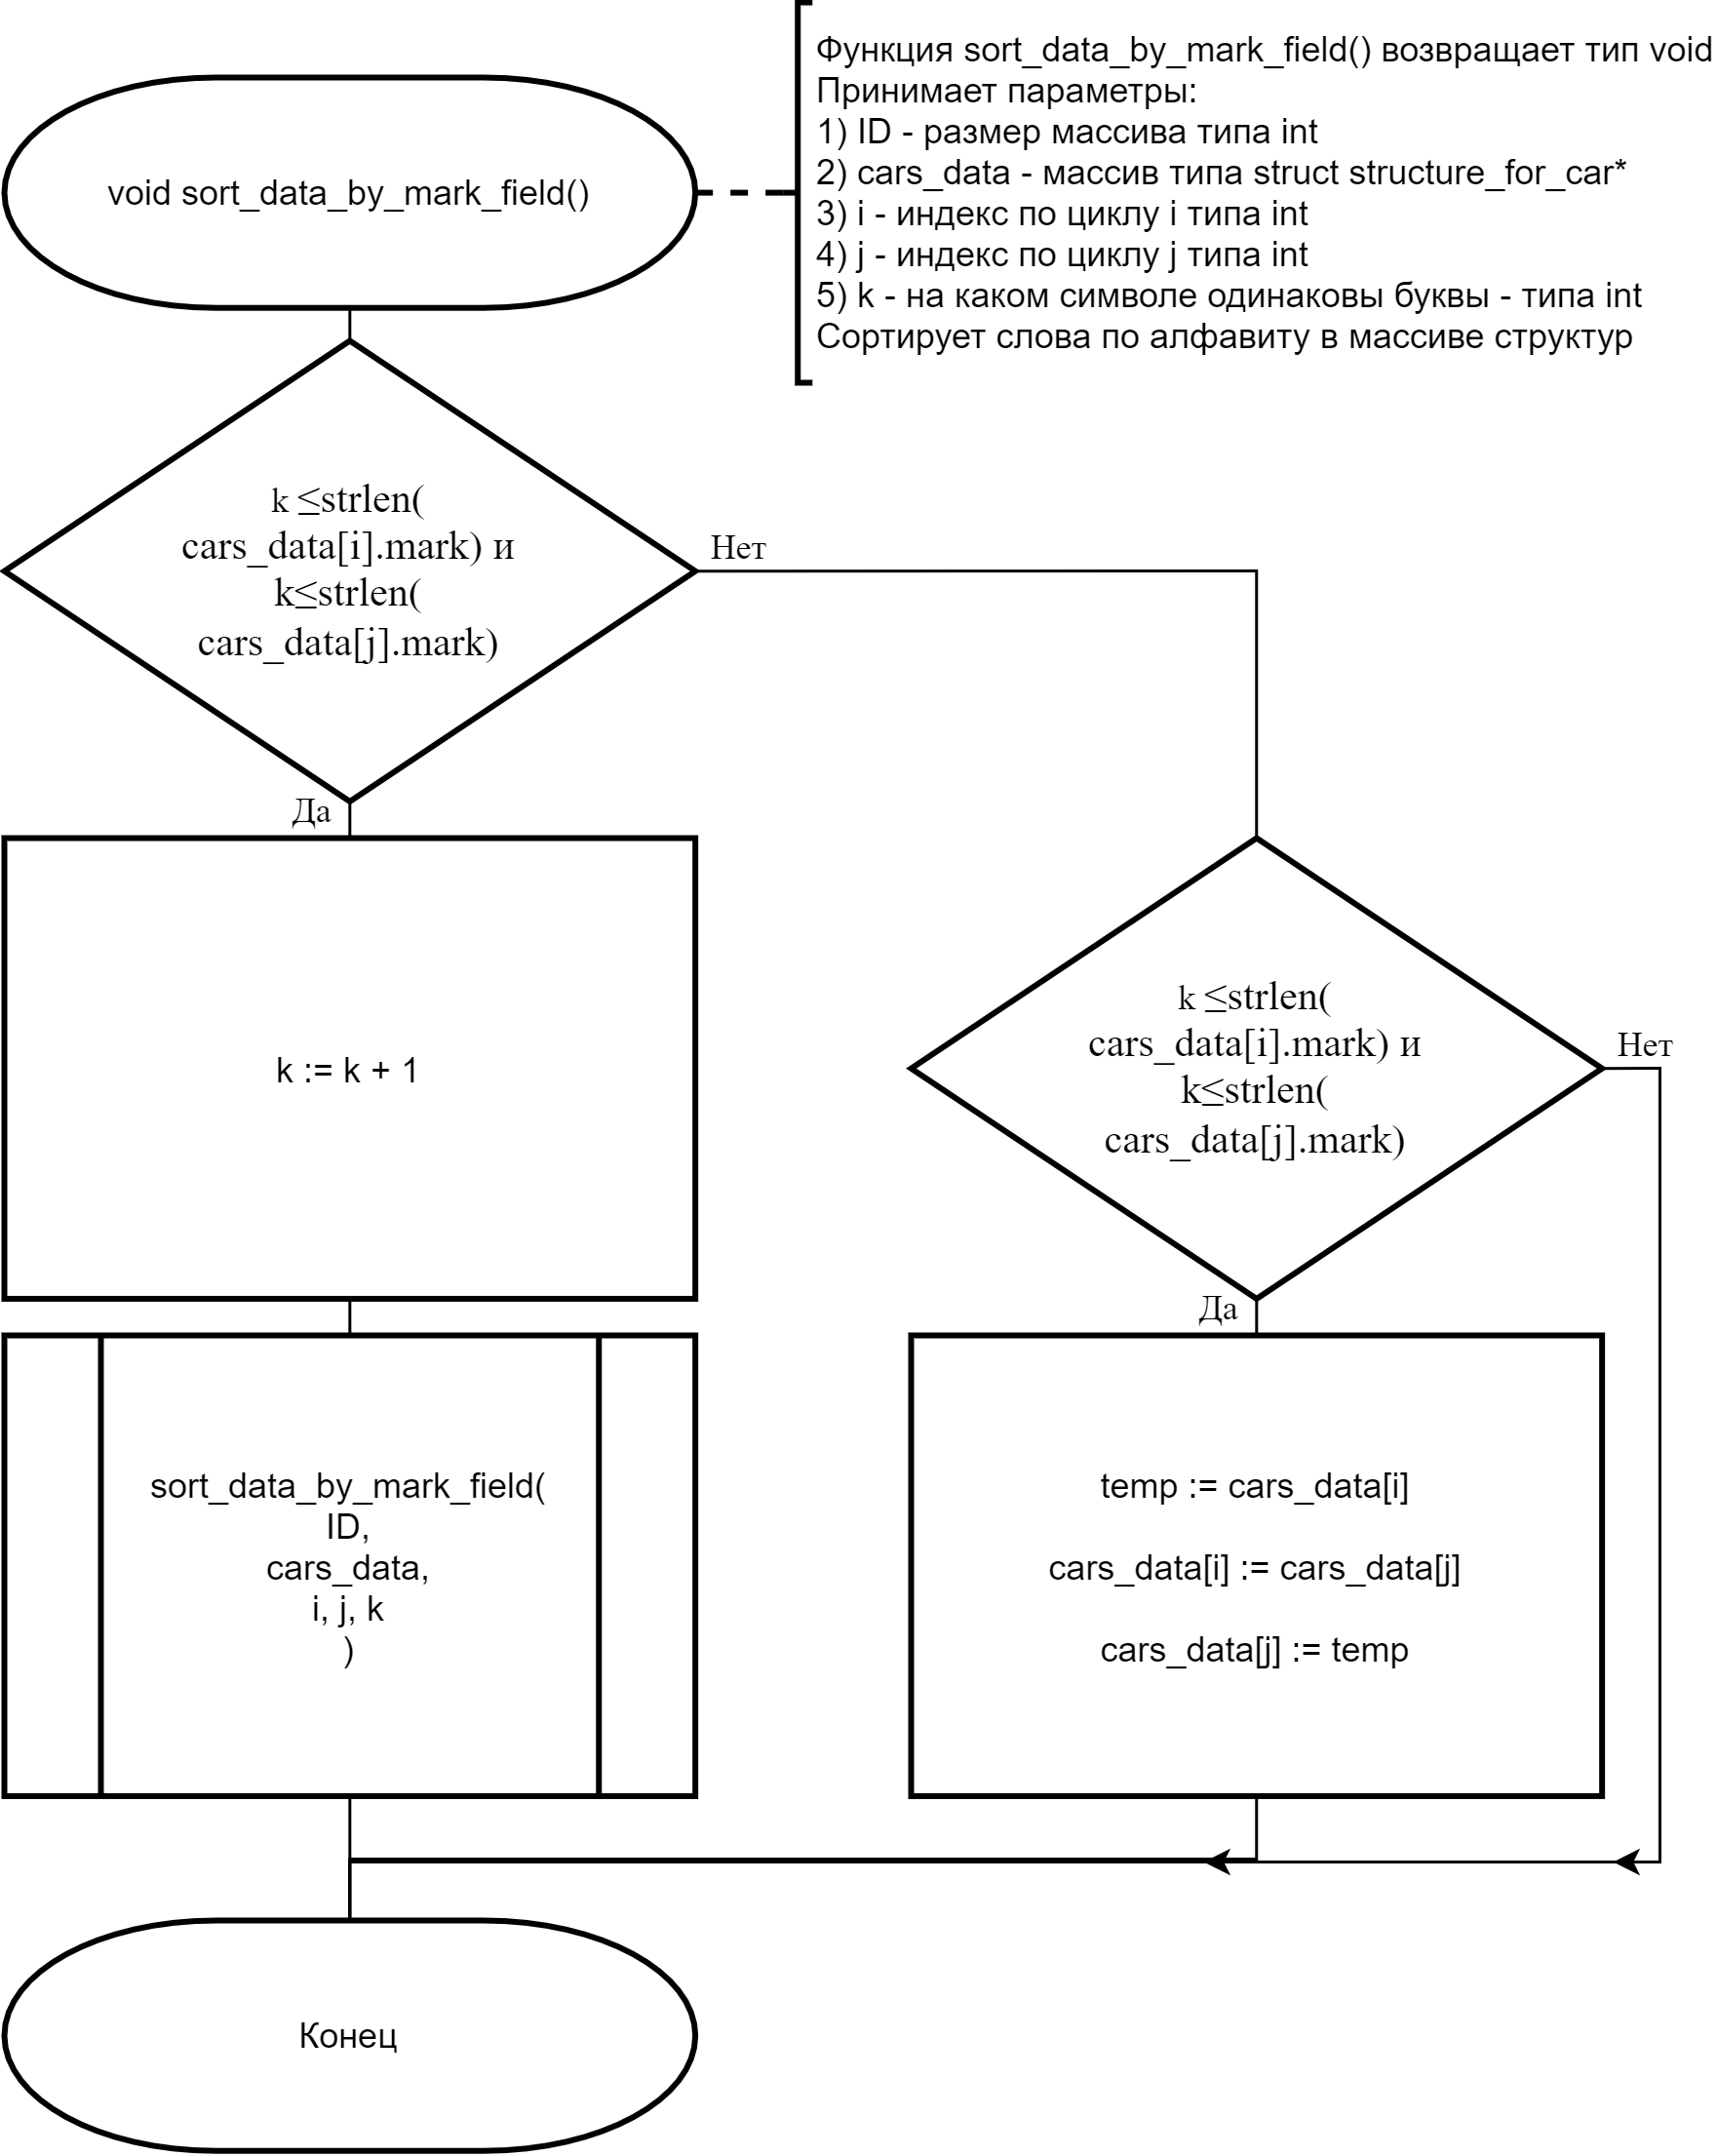
\includegraphics[]{../13/src/lab/menu/sort_data/get_sorted_array/sort_data_by_mark_field/sort_data_by_mark_field.png}
    }
    \caption{sort\_data\_by\_mark\_field()}
    \label{fig:sort_data_by_mark_field}
\end{figure}

\lstinputlisting[
	language=C,
	name=sort\_data\_by\_mark\_field.h
]{../13/src/lab/menu/sort_data/get_sorted_array/sort_data_by_mark_field/sort_data_by_mark_field.h}

\lstinputlisting[
	language=C,
	name=sort\_data\_by\_mark\_field.c
]{../13/src/lab/menu/sort_data/get_sorted_array/sort_data_by_mark_field/sort_data_by_mark_field.c}

\newpage
\subsection{sort\_data\_by\_osmotr\_field()}

\lstinputlisting[
	language=C,
	name=sort\_data\_by\_osmotr\_field.h
]{../13/src/lab/menu/sort_data/sort_data_by_osmotr_field/sort_data_by_osmotr_field.h}

\lstinputlisting[
	language=C,
	name=sort\_data\_by\_osmotr\_field.c
]{../13/src/lab/menu/sort_data/sort_data_by_osmotr_field/sort_data_by_osmotr_field.c}

\newpage
\subsection{sort\_data\_by\_surname\_field()}

Блок-схема на рисунке \ref{fig:sort_data_by_surname_field}.

\begin{figure}[p]
    \center{
        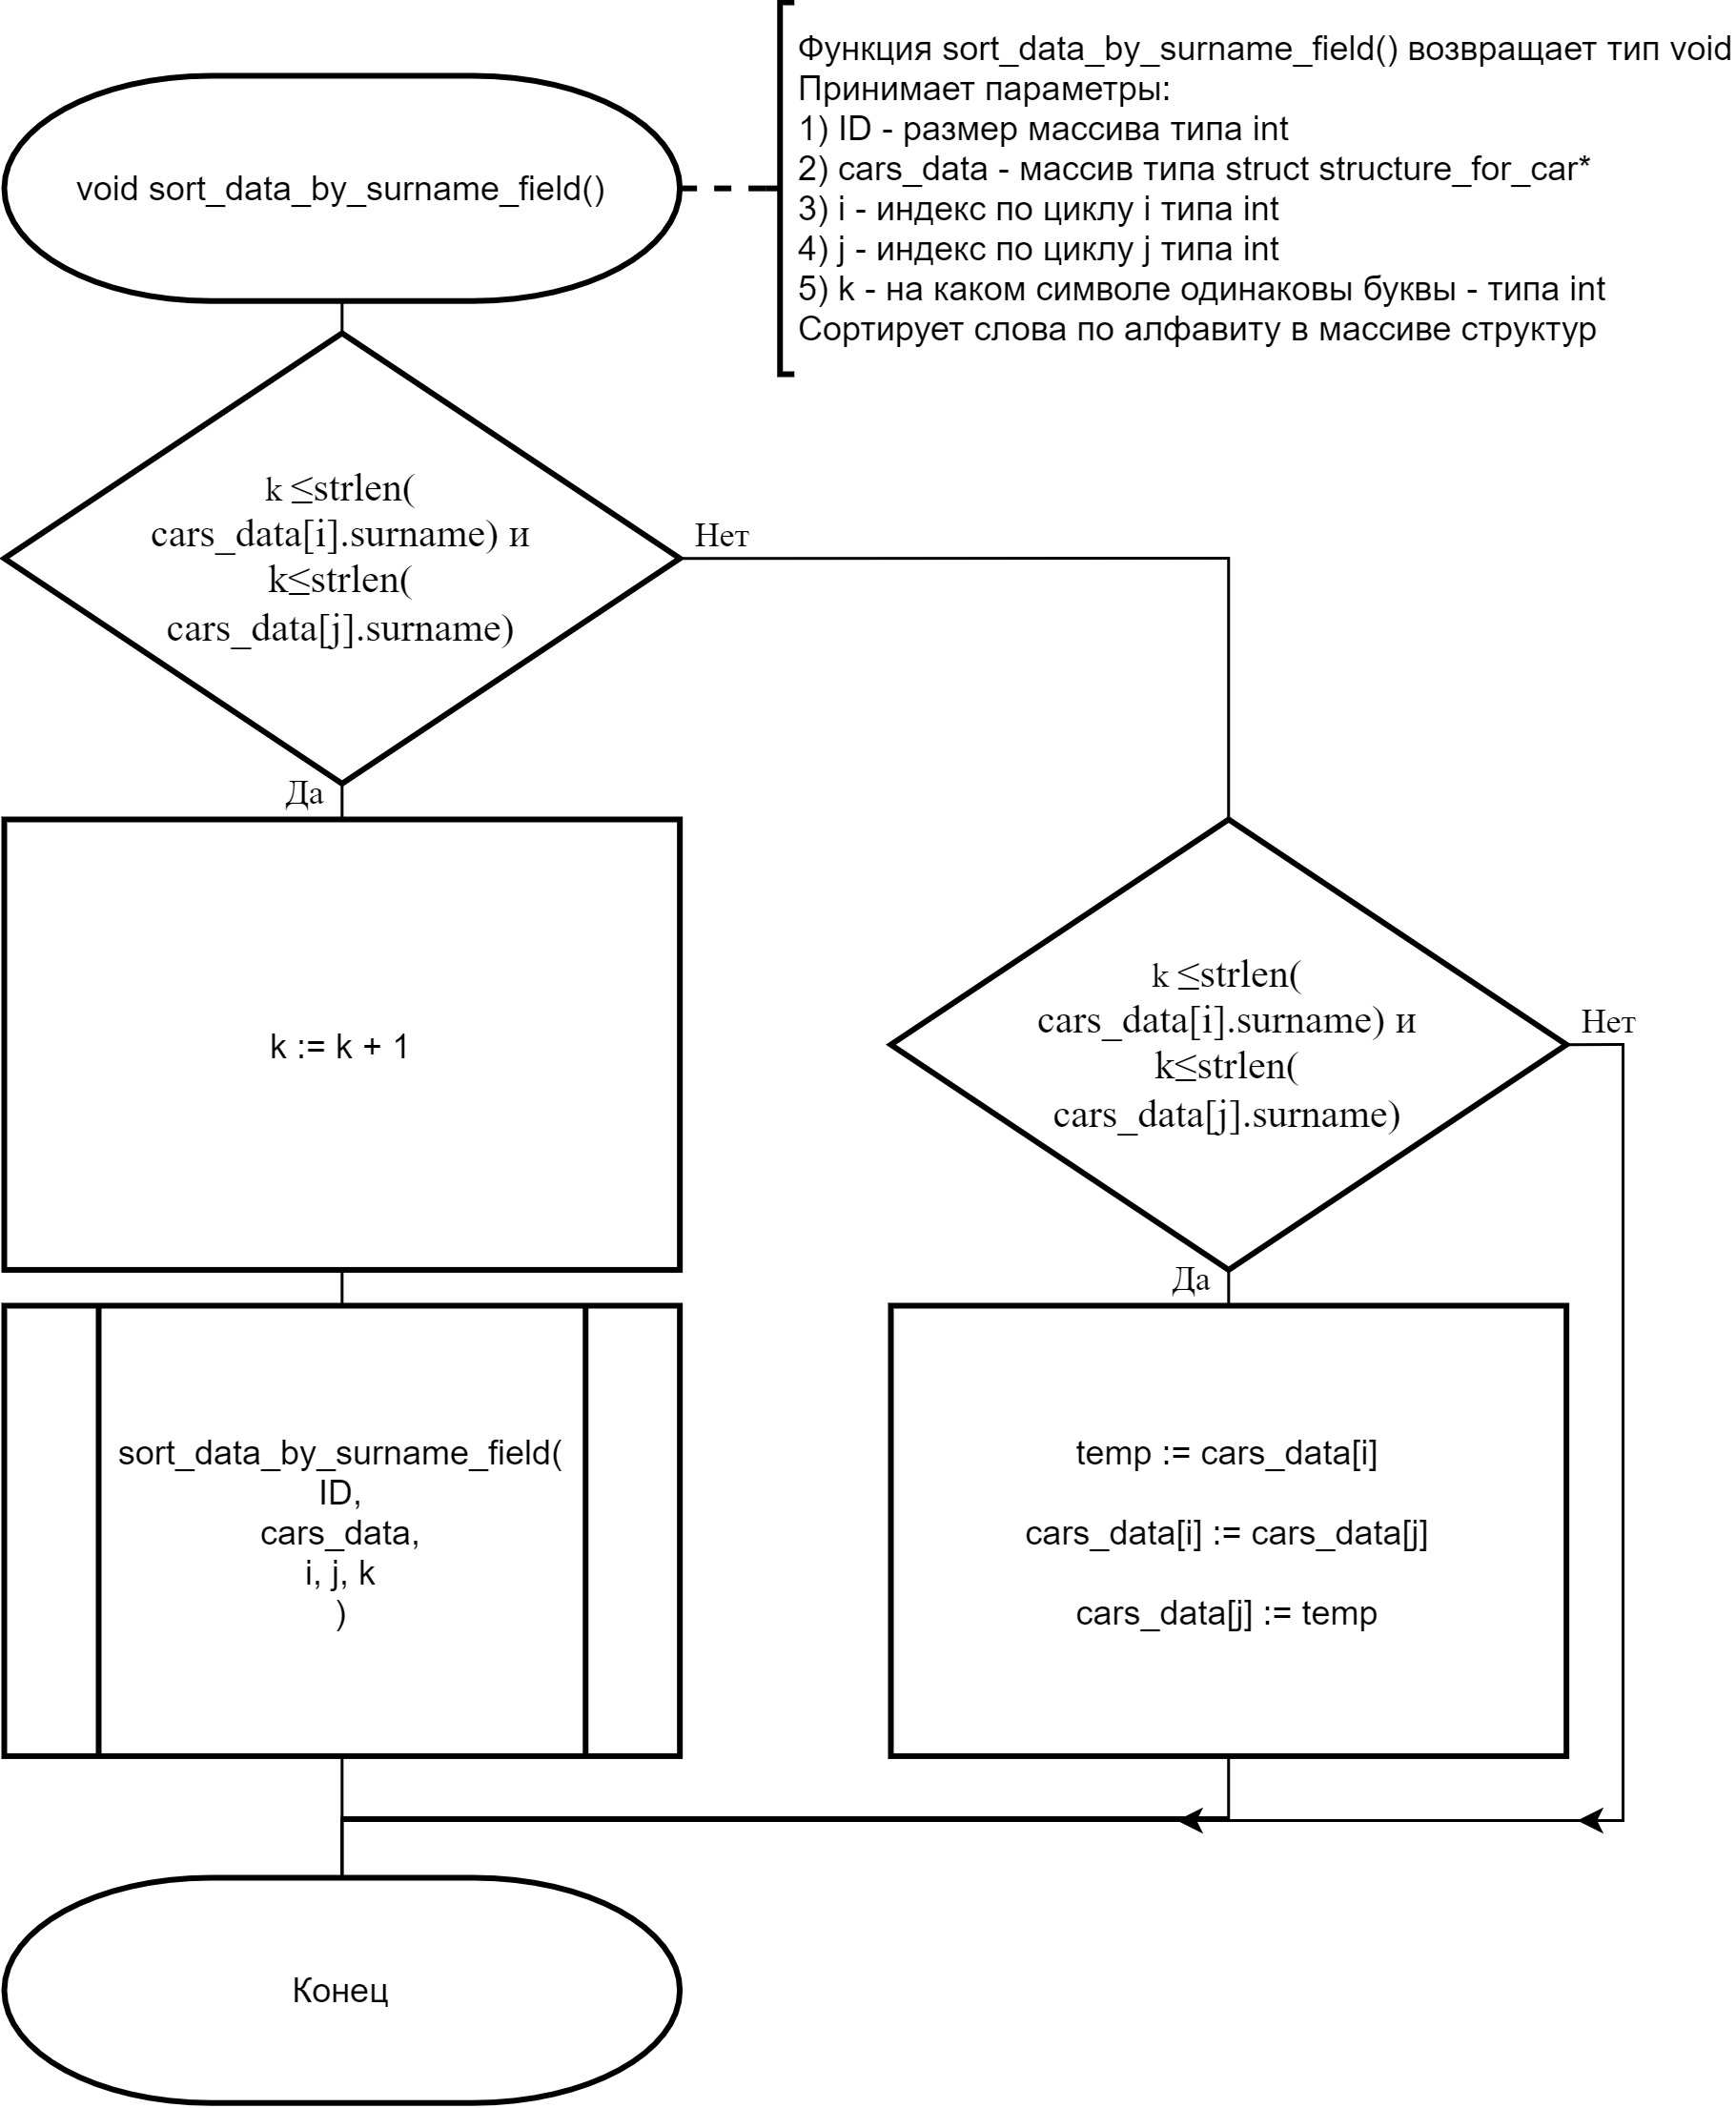
\includegraphics[]{../13/src/lab/menu/sort_data/sort_data_by_surname_field/sort_data_by_surname_field.png}
    }
    \caption{sort\_data\_by\_surname\_field()}
    \label{fig:sort_data_by_surname_field}
\end{figure}

\lstinputlisting[
	language=C,
	name=sort\_data\_by\_surname\_field.h
]{../13/src/lab/menu/sort_data/sort_data_by_surname_field/sort_data_by_surname_field.h}

\lstinputlisting[
	language=C,
	name=sort\_data\_by\_surname\_field.c
]{../13/src/lab/menu/sort_data/sort_data_by_surname_field/sort_data_by_surname_field.c}

\newpage
\subsection{sort\_data\_in\_number\_field()}

Блок-схема на рисунке \ref{fig:sort_data_in_number_field}.

\begin{figure}[p]
    \center{
        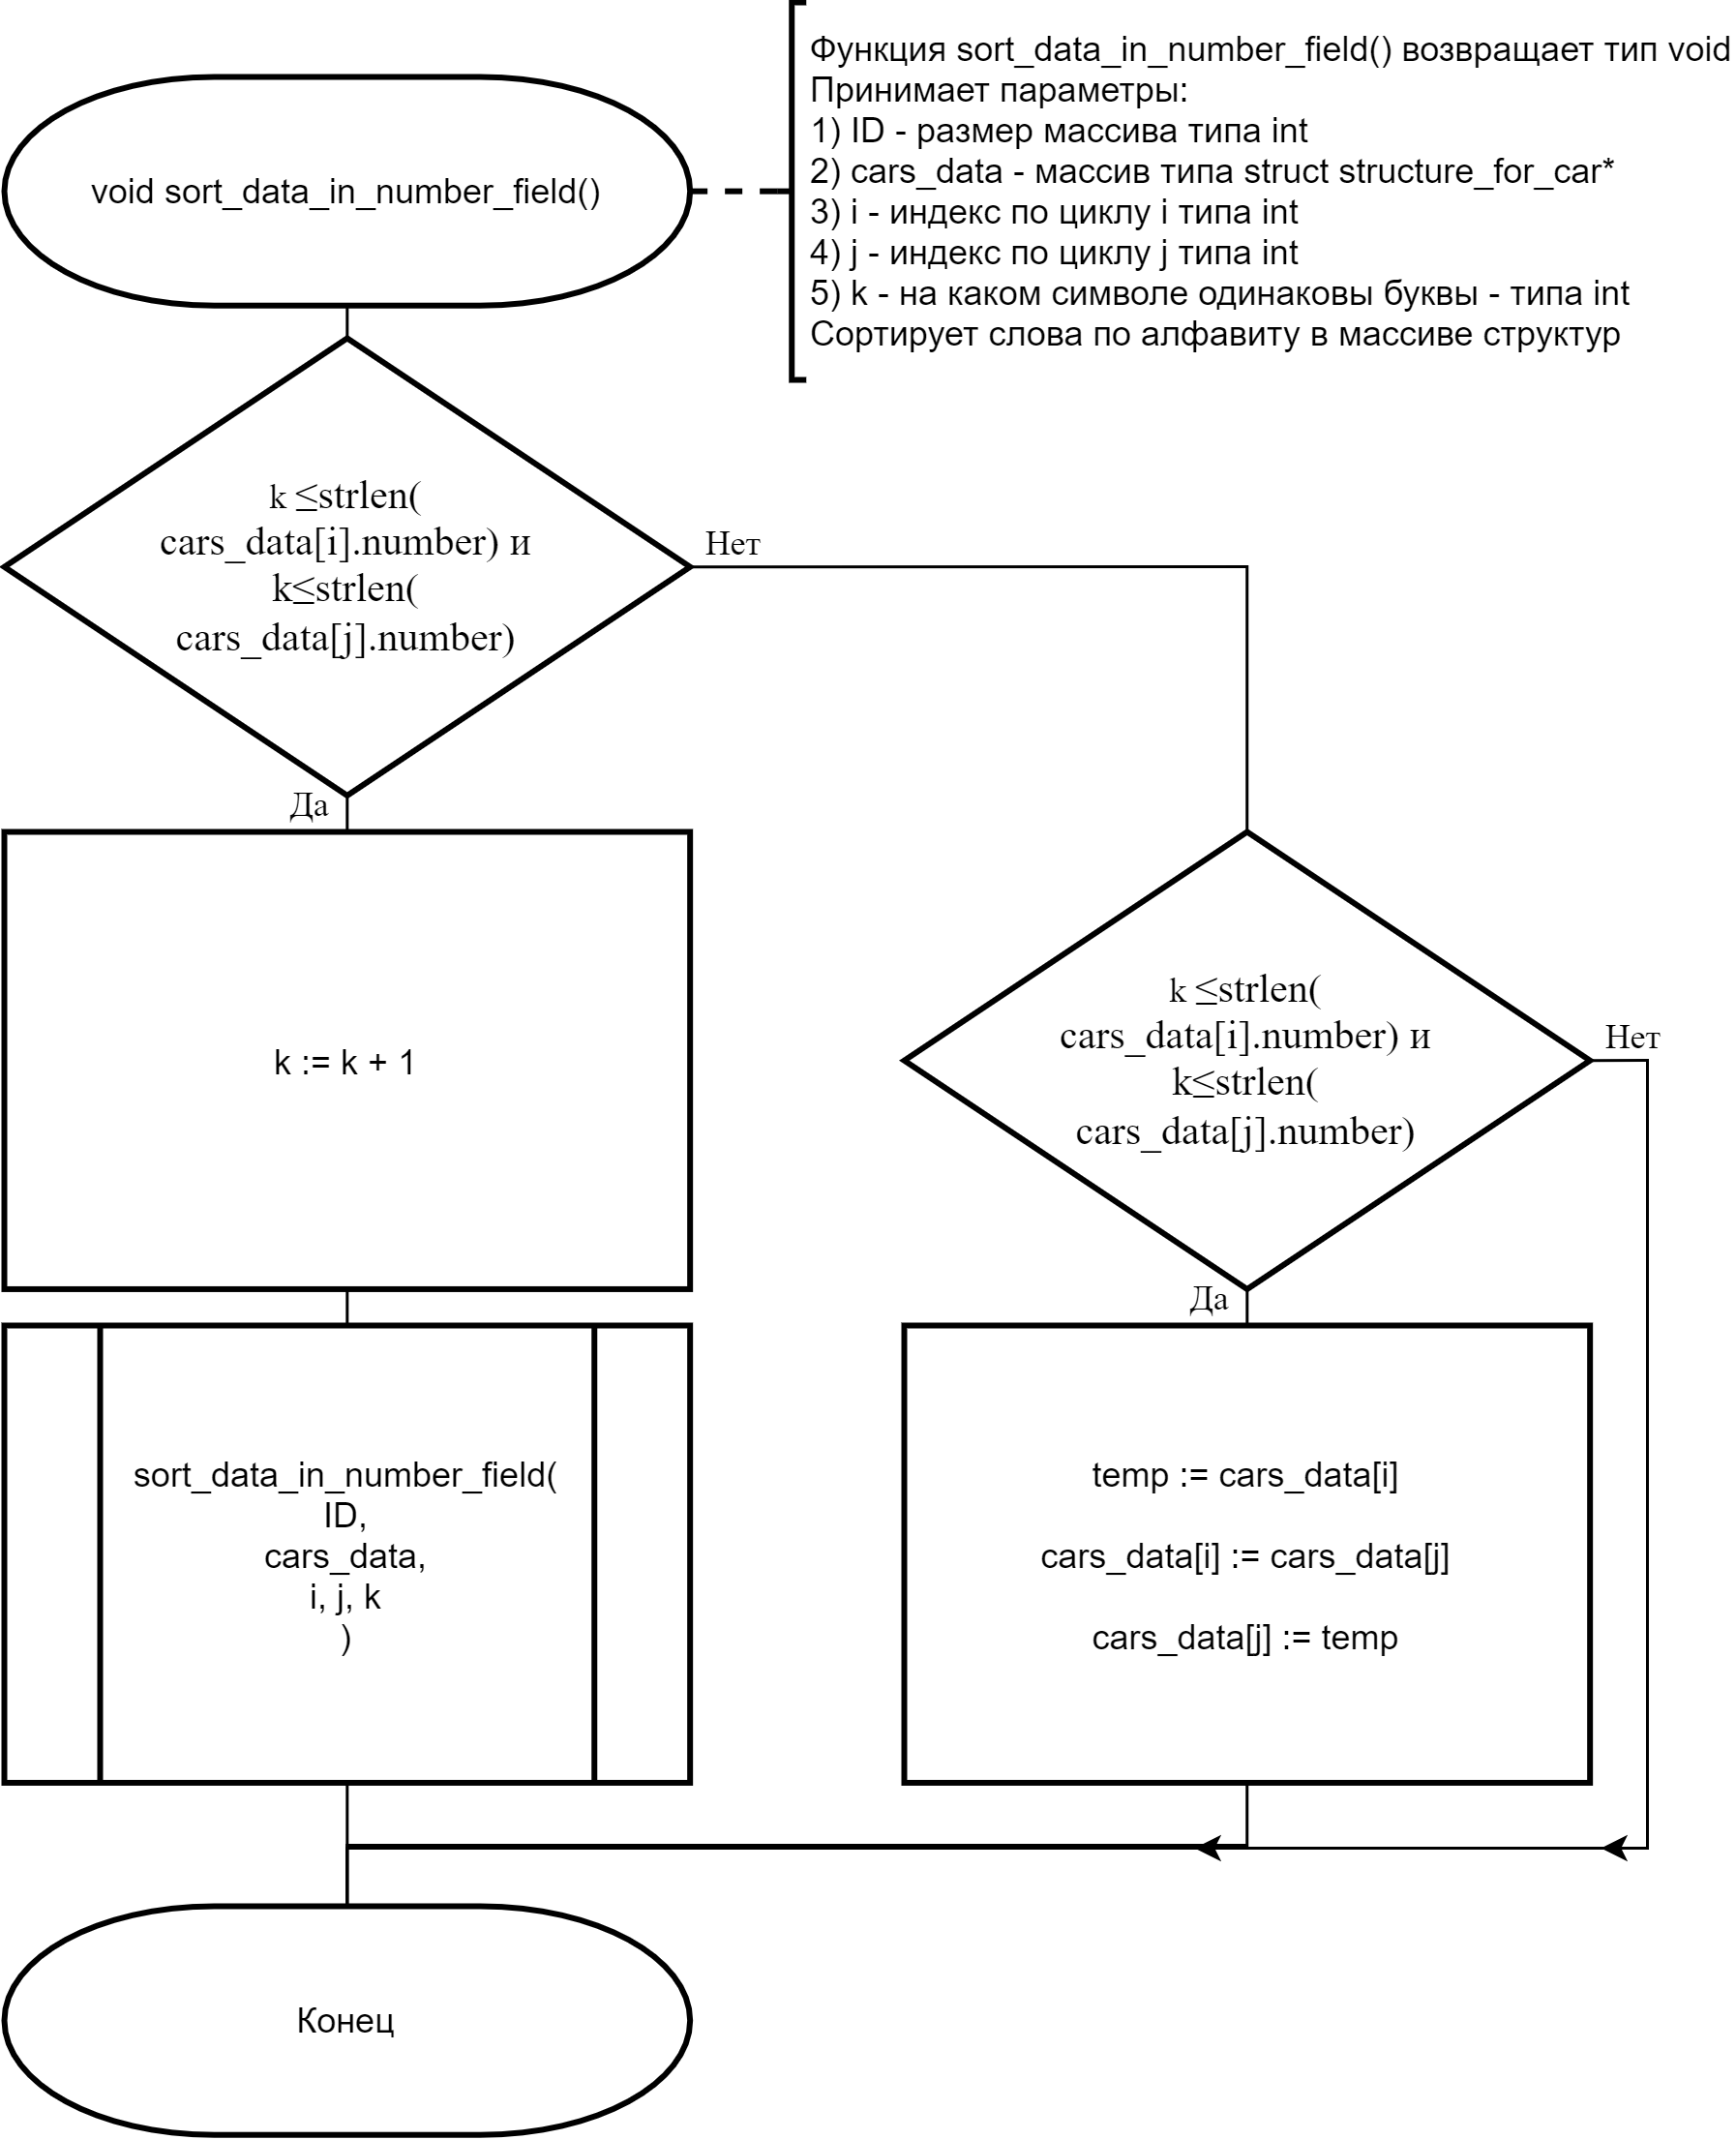
\includegraphics[]{../13/src/lab/menu/sort_data/get_sorted_array/sort_data_in_number_field/sort_data_in_number_field.png}
    }
    \caption{sort\_data\_in\_number\_field()}
    \label{fig:sort_data_in_number_field}
\end{figure}

\lstinputlisting[
	language=C,
	name=sort\_data\_in\_number\_field.h
]{../13/src/lab/menu/sort_data/get_sorted_array/sort_data_in_number_field/sort_data_in_number_field.h}

\lstinputlisting[
	language=C,
	name=sort\_data\_in\_number\_field.c
]{../13/src/lab/menu/sort_data/get_sorted_array/sort_data_in_number_field/sort_data_in_number_field.c}

\newpage
%===>>>

%<<<===Вывод ЛР
%\labconclusion{}
%===>>>

%<<<===Литература
%\newpage
%\begin{thebibliography}{3}
%    \bibitem{}
%\end{thebibliography}
%===>>>

\end{document}